%% ─────────────────────────────────────────────────────────────────
%% СГЕНЕРИРОВАННЫЙ ФАЙЛ — НЕ ПРАВИТЬ РУКАМИ.
%%
%% Подсвеченная версия рукописи (marked-up copy) для related files.
%% Это полная копия main.tex с включённым флагом \markuptrue.
%% Любые правки вносятся в main.tex, после чего:
%%     python scripts/7_revision/20_make_marked.py
%%
%% Синий — новый или переписанный текст
%% Красный зачёркнутый — удалённый фрагмент
%% [REMOVED: ...] — удалённый крупный фрагмент
%% [TODO: ...] — незаполненный слот, виден в обеих версиях
%% ─────────────────────────────────────────────────────────────────
\documentclass{wlscirep}
\usepackage[utf8]{inputenc}
\usepackage[T1]{fontenc}
\usepackage{booktabs}
\usepackage{multirow}
\usepackage{graphicx}
\usepackage{amsmath}
\usepackage{amssymb}
\usepackage{xcolor}
\usepackage{url}
\usepackage{tabularx}
\usepackage{adjustbox}
\usepackage{float}
\usepackage{pifont}
\usepackage[normalem]{ulem}
\usepackage[rightbars,color]{changebar}
\usepackage{lineno}


\definecolor{correct}{RGB}{0,100,200}
\definecolor{incorrect}{RGB}{220,38,38}
\definecolor{hallucinated}{RGB}{22,163,74}

%% ─────────────────────────────────────────────────────────────────
%% Разметка правок ревизии.
%%   \markupfalse — чистая рукопись (файл для основной подачи);
%%   \markuptrue  — подсвеченная версия (marked-up, в related files).
%% Обе версии собираются из ЭТОГО файла: переключается одна строка ниже,
%% ничего больше править не нужно.
%% ─────────────────────────────────────────────────────────────────
\newif\ifmarkup
% Подсвеченная версия собирается БЕЗ правки этого файла: в Overleaf нужно
% выбрать главным документом main_marked.tex — он задаёт \MARKUPVERSION
% и подключает этот же файл. Так обе версии всегда остаются синхронными.
\markuptrue  % включено скриптом 20_make_marked.py

\definecolor{revised}{RGB}{0,90,160}
\definecolor{markerbar}{RGB}{240,170,20}
\setlength{\changebarwidth}{3pt}
\setlength{\changebarsep}{6pt}
% \rev{...}    — новый или переписанный текст
% \del{...}    — удалённый короткий фрагмент (зачёркивание); ТОЛЬКО вне формул,
%                \sout несовместим с математическим режимом
% \delpar{...} — удалённый крупный фрагмент (без зачёркивания: \sout ломается
%                на длинных абзацах с \cite, а проверить сборку локально нельзя)
% Тексты внутри макросов только латиницей: преамбула использует [T1]{fontenc},
% в котором нет кириллицы.
%% Стиль разметки правок:
%%   \markbartrue  — текст остаётся ЧЁРНЫМ, правка отмечается цветной полосой
%%                   на поле (как отчерк маркером). Работает с формулами,
%%                   ссылками и фрагментами длиннее абзаца;
%%   \markbarfalse — правка выделяется синим текстом.
%% Внутри таблиц и рисунков полосу на поле LaTeX не рисует (ограничение
%% плавающих объектов), поэтому там всегда используется цвет — макросы
%% \revf и \revmf.
\newif\ifmarkbar
\markbartrue

\newcommand{\rev}[1]{%
  \ifmarkup
    \ifmarkbar\cbstart#1\cbend\else\textcolor{revised}{#1}\fi
  \else#1\fi}
% \revm{...} — то же для содержимого формул: \textcolor опирается на \leavevmode
%              и в математическом режиме ненадёжен, \color безопасен
\newcommand{\revm}[1]{\ifmarkup\ifmarkbar#1\else{\color{revised}#1}\fi\else#1\fi}
% \revf / \revmf — внутри плавающих объектов: только цвет
\newcommand{\revf}[1]{\ifmarkup\textcolor{revised}{#1}\else#1\fi}
\newcommand{\revmf}[1]{\ifmarkup{\color{revised}#1}\else#1\fi}
\newcommand{\del}[1]{\ifmarkup\textcolor{incorrect}{\sout{#1}}\fi}
\newcommand{\delpar}[1]{\ifmarkup\textcolor{incorrect}{[\textbf{REMOVED:} #1]}\fi}
% \todo{...} — незаполненный слот. Печатается ВСЕГДА, в том числе в чистой версии:
% это защита от подачи с незаполненными данными, а не пометка для себя.
\newcommand{\todo}[1]{\textcolor{incorrect}{\textbf{[TODO: #1]}}}

\title{Two-Stage Synthetic-to-Real Transfer Learning for Automated Mammography Report Generation Using Vision-Language Models}

\author[1]{Gani Esen}
\author[1,2,*]{Marat Nurtas}
\author[3]{Jandos Amankulov}
\author[4]{Laura La Paglia}

\affil[1]{Faculty of Information Technology, International Information Technology University, Almaty 050000, Kazakhstan}
\affil[2] {Faculty of Information Technology and Artificial Intelligence, Al-Farabi Kazakh National University, Almaty 050000, Kazakhstan}
\affil[3]{Department of Radiology and Nuclear Medicine, Kazakh Institute of Oncology and Radiology, Almaty 050051, Kazakhstan}
\affil[4]{Institute for High Performance Computing and Networking (ICAR), National Research Council (CNR) of Italy, Via Ugo La Malfa 153, Palermo 90146, Italy}
\affil[*]{Corresponding author: m.nurtas@iitu.edu.kz}

\keywords{mammography; report generation; vision-language models; low-rank adaptation; equivalence testing; negative result}

%% ─────────────────────────────────────────────────────────────────
%% Второй раунд ревизии. Абстракт перестроен так, чтобы жанр работы был
%% объявлен первыми двумя предложениями (R3.2/R3.4): фреймворк + контролируемая
%% пререгистрированная проверка его синтетической стадии. Все числа переведены
%% на чистое подмножество теста n=49 (R1.2), число прогонов сетки исправлено
%% с 40 на фактические 36 (R3.6).
%% ─────────────────────────────────────────────────────────────────

\begin{abstract}
\rev{We present a two-stage synthetic-to-real transfer learning framework for automated mammography report generation, together with a controlled, preregistered evaluation of whether its synthetic pretraining stage contributes to final report quality.} Automated mammography report generation is constrained by the scarcity of paired mammogram-report data: public collections such as VinDr-Mammo and CBIS-DDSM provide structured annotations but no free-text reports. \rev{The framework converts BI-RADS annotations into synthetic reports (400 generated, 390 retained) to pretrain MedGemma-4B with multimodal LoRA, then fine-tunes on 407 real DMID reports. On the leak-free DMID test subset it reaches ROUGE-L 0.656, METEOR 0.666, CIDEr 0.649 and BERTScore 0.917, exceeding eight baselines and the published state of the art. The evaluation then shows that synthetic pretraining does not produce these numbers: the apparent advantage was measured between models of unequal adapter capacity, and at matched capacity the two schemes are equivalent. Across 36 training runs over three corpus sizes, capacities and initialisations, against a margin fixed in advance, no configuration favours two-stage training; capacity alone reproduces the gap. Two findings bear on evaluation. Under an assertion-level criterion no model fabricates findings; the characteristic error is omission. Textual and clinical quality diverge within one model: where two-stage training gains 0.058 ROUGE-L, BI-RADS agreement and sensitivity both fall. With agreement never exceeding $\kappa = 0.14$, the obstacle to clinically useful reporting is diagnostic accuracy, not fluency.}
\end{abstract}

\begin{document}
\raggedbottom
% цвет полосы задаётся здесь, а не в преамбуле:
% там его перебивали настройки класса
\cbcolor{markerbar}
\maketitle
% Требования Sci Rep к пересмотренной рукописи: арабские номера
% страниц в колонтитуле и номера строк для удобства рецензентов
\thispagestyle{plain}
\pagestyle{plain}
\linenumbers

% Шапка подсвеченной версии. Видна ТОЛЬКО при \markuptrue, поэтому служит
% индикатором: если её нет, значит собирается чистая версия.
\ifmarkup
  \begin{center}
  \fcolorbox{revised}{white}{\parbox{0.93\linewidth}{\small
  \textbf{MARKED-UP COPY.}
  \ifmarkbar
  Text added or rewritten in this revision is marked by a
  \textcolor{markerbar}{\rule{9pt}{3pt}} bar in the outer margin;
  the text itself is unchanged in colour.
  Inside tables and figure captions the margin bar is unavailable, so
  revised text there is shown \textcolor{revised}{in blue} instead.
  \else
  Text added or rewritten in this revision is shown
  \textcolor{revised}{in blue}.
  \fi
  \textcolor{incorrect}{\sout{Deleted text is struck through in red}}
  and larger deletions are summarised as
  \textcolor{incorrect}{[REMOVED: \ldots]}.
  \textcolor{incorrect}{\textbf{[TODO: \ldots]}} marks a slot that is still to be
  filled and appears in both versions.
  The clean manuscript is produced from the same source by compiling
  \texttt{main.tex} instead of \texttt{main\_marked.tex}.}}
  \end{center}
  \vspace{0.6em}
\fi


%% ─────────────────────────────────────────────────────────────────
\section*{Introduction}
%% ─────────────────────────────────────────────────────────────────

Breast cancer remains the most commonly diagnosed cancer worldwide, with approximately 2.3 million new cases in 2022 and representing the leading cause of cancer-related mortality in women~\cite{bray2024global}. Mammography remains the gold standard for population-level breast cancer screening, with evidence demonstrating that regular screening reduces breast cancer mortality by 20--40\% through early-stage detection~\cite{lehman2015mammographic, sechopoulos2021artificial}. However, the clinical utility of mammography is fundamentally constrained by two interrelated challenges: a global shortage of trained radiologists and the high cognitive burden of interpreting large volumes of screening examinations.

Deep learning has shown remarkable success in medical imaging~\cite{esteva2019guide}, including mammography-based cancer detection~\cite{mckinney2020international, lotter2021robust, shen2019deep} and risk prediction~\cite{yala2019deep}. Radiologists are required to produce standardised structured reports following the Breast Imaging Reporting and Data System (BI-RADS) lexicon developed by the American College of Radiology~\cite{birads2013}. These reports must accurately characterise breast density~\cite{gastounioti2022breast, lehman2019mammographic}, describe identified findings (masses, calcifications, architectural distortions, asymmetries), assign a BI-RADS assessment category (0--6), and specify a management recommendation. Report generation is time-intensive, and inter-reader variability remains a persistent limitation. Automated report generation systems that assist radiologists by producing structured report drafts represent a high-value clinical application.

Recent advances in Vision-Language Models (VLMs) have demonstrated remarkable capabilities in generating natural language descriptions from medical images~\cite{wang2024mllm_survey}. Models such as LLaVA-Med~\cite{li2024llavamed}, BiomedCLIP~\cite{zhang2023biomedclip}, and MedGemma~\cite{lin2024medgemma} have shown strong performance on radiology report generation, particularly for chest X-ray interpretation using the MIMIC-CXR dataset~\cite{johnson2019mimiccxr}. Large language models such as Med-PaLM~\cite{singhal2023medpalm} have demonstrated clinical-level knowledge, while Med-Flamingo~\cite{moor2023medflamingo} explored few-shot medical reasoning. However, mammography remains significantly underexplored within the VLM literature. Unlike chest radiography, mammography presents unique challenges: high-resolution full-field digital images requiring fine-grained lesion characterisation, the clinical necessity of multi-view reasoning across craniocaudal (CC) and mediolateral oblique (MLO) projections, and a domain-specific reporting vocabulary governed by the BI-RADS lexicon.

The central obstacle to developing VLMs for mammography report generation is the absence of large-scale publicly available paired datasets---collections of mammographic images matched with corresponding narrative radiology reports. While several public mammography datasets exist, including CBIS-DDSM~\cite{lee2017curated} and VinDr-Mammo~\cite{nguyen2023vindr}, these resources provide structured annotations rather than free-text radiology reports. Only the Digital Mammography Dataset for Breast Cancer Diagnosis Research (DMID)~\cite{oza2024} provides a modest collection (225 cases, 510 images) of paired images and narrative reports; all other publicly accessible mammography datasets lack this critical pairing. Aitimov et al.~\cite{aitimov2025feature} recently developed feature extraction methods for breast cancer detection on VinDr-Mammo using modified Faster R-CNN, demonstrating growing interest in computational mammography from the Central Asian research community.

Our prior work explored dimensionality reduction for breast cancer classification~\cite{esen2024pca}, multi-task attention-guided architectures for joint pathology and density estimation in mammography~\cite{esen2025multitask}, and reinforcement learning with visual interpretability for breast cancer diagnosis~\cite{esen2025rl}. The current work extends this line of research from classification to automated report generation.

\rev{To address the data scarcity challenge, we propose a two-stage synthetic-to-real transfer learning framework for automated mammography report generation, and subject it to a controlled evaluation of whether its synthetic stage is what makes it work.} Our contributions are:

\begin{enumerate}
  \item We introduce a \textbf{scalable label-to-report synthesis pipeline} that converts publicly available structured mammography annotations into synthetic training reports, with automated validation of BI-RADS mention, recommendation presence and minimum length. We release the corpus together with an audit of its defects, including 5.4\% of reports generated in the wrong language and passed by the validator.
  \item \rev{We report the \textbf{first preregistered equivalence evaluation of synthetic pretraining in medical report generation}: two one-sided tests on a margin fixed before any run was executed, over 36 training runs spanning three corpus sizes, three adapter capacities and three initialisations. We release the resulting benchmark---the per-sample generations underlying the primary analyses, the leak-free test subset, and the scripts that compute every table---so that the evaluation itself can be reused.}
  \item \rev{We give a \textbf{measured decomposition of an apparent transfer-learning gain into four confounds}---adapter capacity, evaluation prompt, transfer mechanism and a single initialisation---each quantified separately on the same models. The procedure is a reusable template for auditing a published effect without re-running the original system.}
  \item \rev{We provide a \textbf{clinical analysis at matched capacity} showing that these models do not fabricate findings but omit them, that omission affects between a third and a half of the cases whose reference asserts a finding, and that BI-RADS agreement does not exceed $\kappa = 0.14$ for any model evaluated. An offline reader-study instrument is released with the code so that expert adjudication can be added to this benchmark.}
  \item We document a \textbf{divergence between textual and clinical quality within a single model}: at small adapter rank two-stage training gains 0.058 ROUGE-L ($p=0.0001$) while losing BI-RADS agreement and finding sensitivity. We argue from this that $n$-gram overlap should not be used to select mammography report generators.
\end{enumerate}

%% ─────────────────────────────────────────────────────────────────
\section*{Related Work}
%% ─────────────────────────────────────────────────────────────────

\subsection*{Automated Radiology Report Generation}

Automated radiology report generation has been studied extensively for chest X-ray interpretation, where large paired image-report datasets such as MIMIC-CXR~\cite{johnson2019mimiccxr} have enabled supervised learning. Early methods relied on CNN-LSTM architectures with attention mechanisms, while more recent approaches leverage transformer-based~\cite{vaswani2017attention} encoder-decoder frameworks. R2Gen~\cite{chen2020r2gen} introduced a relational memory-driven decoder, while R2GenCMN~\cite{chen2022r2gencmn} extended this with cross-modal memory networks. Miura et al.~\cite{miura2021improving} addressed factual completeness and consistency in report generation. PromptMRG~\cite{jin2024promptmrg} introduced diagnosis-driven prompts for medical report generation. CT2Rep~\cite{hamamci2024ct2rep} extended automated report generation to 3D medical imaging. Despite these advances, mammography remains largely unaddressed due to data scarcity.

\subsection*{Vision-Language Models for Mammography}

Vision-language models such as CLIP~\cite{radford2021clip} and its medical adaptations BiomedCLIP~\cite{zhang2023biomedclip} have enabled multimodal understanding of medical images. LLaVA~\cite{liu2024llava} and its medical variant LLaVA-Med~\cite{li2024llavamed} demonstrated visual instruction tuning for medical question answering.

For mammography specifically, Mammo-CLIP~\cite{ghosh2024} introduced the first VLM pretrained on screening mammogram-report pairs. MV-MLM~\cite{ahmed2025} extended this with multi-view contrastive learning using synthetic text reports. AMRG~\cite{sung2025} established the first reproducible benchmark for mammography report generation, fine-tuning MedGemma-4B with LoRA~\cite{hu2022lora} on the DMID dataset and achieving ROUGE-L of 0.569, METEOR of 0.615, and CIDEr of 0.582, with systematic LoRA hyperparameter exploration across five VLM backbones. MammoWise~\cite{jahangir2026} proposed a local multi-model RAG pipeline with QLoRA~\cite{dettmers2024qlora} fine-tuning achieving BI-RADS accuracy of 0.755. \rev{Our work introduces a two-stage training paradigm, and a controlled evaluation of whether its synthetic stage is responsible for the scores it obtains on the DMID benchmark.}

\subsection*{Transfer Learning in Medical Imaging}

Transfer learning from large-scale pretraining to domain-specific fine-tuning has become the dominant paradigm in medical image analysis~\cite{pan2010transfer, zhuang2021survey}. Deep representation learning~\cite{bengio2012deep} enables models to extract transferable features across domains. Modern architectures such as ResNet~\cite{he2016deep}, DenseNet~\cite{huang2017densely}, and the Vision Transformer~\cite{dosovitskiy2021vit} have been foundational to progress in medical image analysis, and hybrid attention-transformer designs such as DA-TransUNet~\cite{sun2024datransunet} continue to advance dense prediction tasks in this domain. In radiology, models pretrained on general image-text data are typically fine-tuned on domain-specific datasets. However, when paired data is unavailable, alternative pretraining strategies are needed. Our two-stage framework can be viewed through a curriculum learning lens: Stage~1 (synthetic data) provides a simpler learning signal with consistent formatting, while Stage~2 (real data) introduces the complexity and variability of authentic radiologist reports. Recent advances have also explored graph-based architectures for medical applications where high-order biological relationships are critical, such as heterogeneity-aware hypergraph neural networks for cancer driver gene identification~\cite{chen2026dprehgnn}, which leverage dual-path residual fusion to integrate multi-omics features with learned hypergraph representations. Such approaches demonstrate the value of capturing high-order associations in data-scarce clinical domains\rev{---a principle that also motivated the retrieval component we tested in mammography}. This synthetic-to-real curriculum has not been previously explored for medical report generation.

\subsection*{Retrieval-Augmented Generation in Healthcare}

Retrieval-Augmented Generation (RAG)~\cite{lewis2020rag} augments generative models by retrieving relevant context from an external knowledge base at inference time, using efficient similarity search such as FAISS~\cite{johnson2020faiss}. In the medical domain, RAG has demonstrated significant benefits for clinical accuracy. \rev{Retrieval can also be made specific to what a report has to express: RADAR~\cite{pan2026radar} retrieves difference-aware, organ-level aligned evidence in order to describe \emph{change} between a prior and a current study, which is the retrieval target in longitudinal reporting.} Our work applies RAG specifically to mammography report generation, grounding generation in the ACR BI-RADS clinical knowledge base~\cite{birads2013} with sentence embeddings via Sentence-BERT~\cite{reimers2019sentencebert}\rev{; the module is ablated rather than adopted, and the ablation is negative (see Retrieval Ablation)}.

\subsection*{Synthetic Data for Medical AI}

The use of LLM-generated synthetic data to overcome annotation scarcity is increasingly validated. MV-MLM demonstrated that VLMs trained on LLM-generated pseudo-reports can outperform fully supervised baselines~\cite{ahmed2025}. \rev{Our work tests that paradigm in the report-generation setting: whether synthetic reports used as pretraining data measurably improve a subsequent real-data fine-tuning stage, at matched capacity and across initialisations.}

\subsection*{Summary of Related Approaches}

Table~\ref{tab:related} summarises the key differences between our approach and prior mammography report generation methods.

\begin{table}[H]
\centering
\caption{Comparison of mammography report generation approaches. Ours is the only method combining synthetic pretraining with real-data fine-tuning. \revf{The RAG column records the inference-time configuration of each method.}}
\label{tab:related}
\small
\begin{tabular}{lccccc}
\toprule
\textbf{Method} & \textbf{Base Model} & \textbf{Paired Data} & \textbf{Synthetic} & \textbf{RAG} & \textbf{Multi-VLM} \\
\midrule
Mammo-CLIP~\cite{ghosh2024} & CLIP & Private & No & No & No \\
MV-MLM~\cite{ahmed2025} & Custom & Private & Yes & No & No \\
AMRG~\cite{sung2025} & MedGemma & DMID & No & No & Yes \\
MammoWise~\cite{jahangir2026}& Multiple & DMID & No & Yes & Yes \\
\textbf{Ours} & MedGemma & DMID & \textbf{Yes} & \revf{No$^{\dagger}$} & \textbf{Yes} \\
\bottomrule
\end{tabular}

\revf{\footnotesize $^{\dagger}$Retrieval was implemented and ablated: it degrades generation and is not used at inference (negative result, see Retrieval Ablation).}
\end{table}

\rev{Our framework combines synthetic data generation with comprehensive multi-model evaluation within a two-stage training paradigm; retrieval was implemented alongside it and is reported as an ablated component rather than as part of the pipeline.} While AMRG and MammoWise evaluate multiple VLM backbones, neither incorporates synthetic pretraining. MV-MLM uses synthetic reports but for classification rather than report generation, and relies on private paired data for evaluation.

%% ─────────────────────────────────────────────────────────────────
\section*{Methods}
%% ─────────────────────────────────────────────────────────────────

\rev{Our framework consists of three components: (1) label-to-report synthesis, (2) Stage~1 synthetic pretraining, and (3) Stage~2 real-data fine-tuning. A BI-RADS retrieval module was implemented alongside them, ablated, and found to degrade generation; it is described at the end of this section and is not part of the pipeline.} Figure~\ref{fig:pipeline} illustrates the architecture.
At a high level, our framework addresses mammography data scarcity by decoupling domain learning into two complementary phases. In the first phase, we generate a large corpus of synthetic reports by converting structured BI-RADS annotations from VinDr-Mammo and CBIS-DDSM into free-text reports using a large language model, then use these pairs to pretrain a multimodal LoRA adapter on top of the MedGemma-4B backbone. This phase teaches the model the vocabulary, structure, and clinical conventions of mammography reporting. In the second phase, the pretrained adapter is further fine-tuned on the smaller set of real radiologist reports from the DMID dataset, which refines the model's output style to match authentic clinical language. Each component is described in detail in the following subsections.

\begin{figure}[H]
\centering
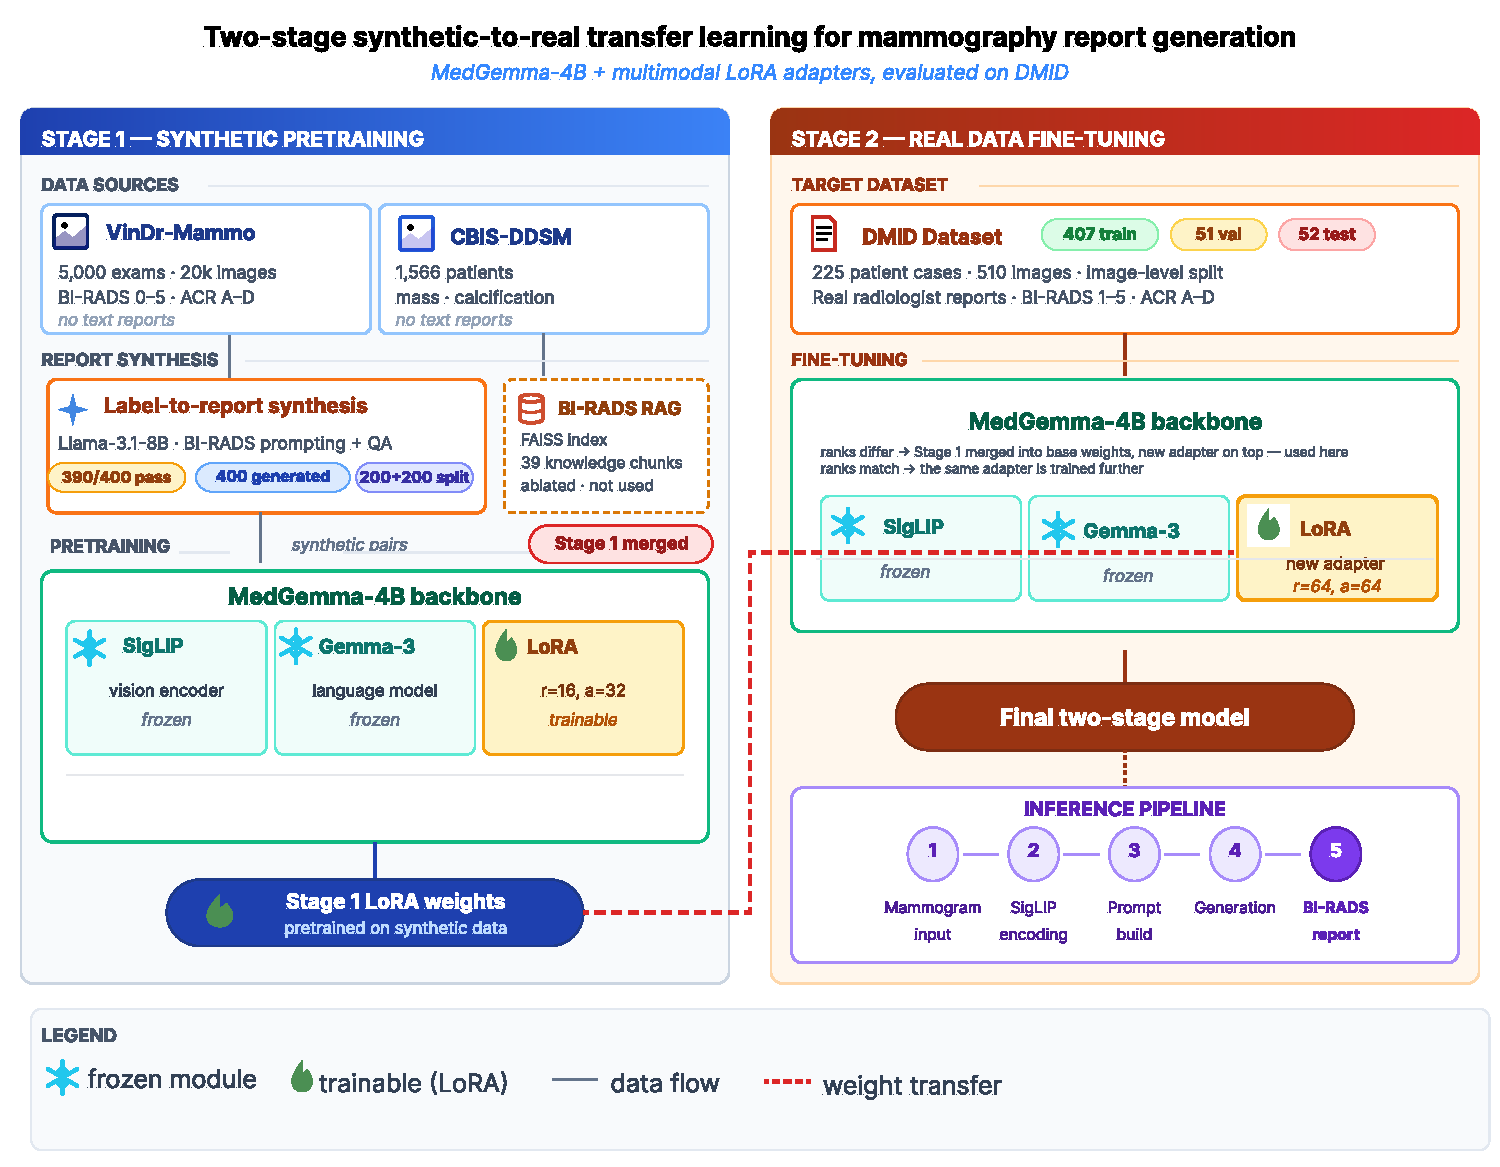
\includegraphics[width=\textwidth]{fig_pipeline_figma.pdf}
\caption{Overview of the two-stage synthetic-to-real transfer learning framework. Stage~1 pretrains on synthetic reports generated from structured BI-RADS annotations in VinDr-Mammo and CBIS-DDSM: 400 reports are generated and 390 pass automated validation (97.5\%). Stage~2 transfers the pretrained LoRA weights and fine-tunes on real radiologist reports from DMID\revf{. Two transfer mechanisms exist---continued training of the same adapter when the Stage~1 and Stage~2 ranks match, or merging Stage~1 into the base weights (Eq.~\ref{eq:merge}) and training a new adapter when they do not}. The BI-RADS retrieval module is shown as ablated and is not part of the inference path: the retrieval ablation shows that it degrades generation, and it is reported as a negative result.}
\label{fig:pipeline}
\end{figure}

\subsection*{Datasets}

We use three publicly available mammography datasets (Table~\ref{tab:datasets}).

\begin{table}[H]
\centering
\caption{Dataset characteristics. Only DMID contains paired free-text radiology reports.}
\label{tab:datasets}
\begin{tabular}{lccccc}
\toprule
\textbf{Dataset} & \textbf{Cases} & \textbf{Images} & \textbf{BI-RADS} & \textbf{Density} & \textbf{Reports} \\
\midrule
VinDr-Mammo~\cite{nguyen2023vindr} & 5,000 & 20,000 & 0--5 & A--D & \textcolor{red}{No} \\
CBIS-DDSM~\cite{lee2017curated} & 1,566 & --- & 0--5 & --- & \textcolor{red}{No} \\
DMID~\cite{oza2024} & 225 & 510 & 1--5 & A--D & \textcolor{hallucinated}{\textbf{Yes}} \\
\bottomrule
\end{tabular}
\end{table}

\textbf{VinDr-Mammo}~\cite{nguyen2023vindr} contains 5,000 four-view screening examinations with breast-level BI-RADS categories, ACR density categories, and finding-level annotations with bounding boxes. \textbf{CBIS-DDSM}~\cite{lee2017curated} contains 1,566 patients with mass and calcification annotations. The INbreast dataset~\cite{moreira2012inbreast}, used in our prior multi-task work~\cite{esen2025multitask}, provides additional mammographic data but also lacks free-text reports. Neither VinDr-Mammo nor CBIS-DDSM contains free-text reports; both are used for Stage~1. \textbf{DMID}~\cite{oza2024} contains 225 cases with paired reports. Following AMRG~\cite{sung2025}, we split DMID into 407 training, 51 validation, and 52 test image-report pairs.

\textbf{Split granularity and leakage.} The split is \emph{image-level}, not patient-level: DMID distributes 510 images over 225 cases, and the image-to-patient mapping is not published, so a patient-level split cannot be reconstructed from the released files (grouping images by identical report text recovers only 59 complete blocks out of 127). We retain the image-level protocol for comparability with AMRG~\cite{sung2025}, and quantify its consequences rather than leaving them implicit. Grouping the 510 reports by normalised text shows that 3 of the 52 test images (Img462, Img464, Img506) have a report that appears verbatim in the training split. \rev{All results below are reported on the leak-free subset of the remaining $49$ test images, which we take as the primary test set; the full $52$-image split is retained only as a sensitivity analysis, where every fine-tuned model scores $0.014$--$0.015$ ROUGE-L higher and no comparison changes.} A per-image split assignment for all 510 images is provided in Supplementary Table~S1.

\subsection*{Label-to-Report Synthesis Pipeline}

Given a mammographic image $\mathbf{x}_i$ with structured annotations $\mathbf{a}_i = (l_i, v_i, d_i, f_i, b_i, c_i)$ representing laterality, view position, ACR density, finding categories, BI-RADS assessment, and bounding box coordinates, we construct a structured prompt $\mathbf{p}_i = \phi(\mathbf{a}_i)$ and generate the synthetic report $\hat{r}_i = \mathcal{G}(\mathbf{p}_i)$ using Llama-3.1-8B~\cite{dubey2024llama3} via local inference (Ollama). Each report undergoes quality validation:
\begin{equation}
\mathcal{V}(\hat{r}_i) = \mathbb{1}[\text{BIRADS}(\hat{r}_i)] \cdot \mathbb{1}[\text{Rec}(\hat{r}_i)] \cdot \mathbb{1}[|\hat{r}_i| \geq \tau]
\label{eq:validation}
\end{equation}
where $\mathbb{1}[\cdot]$ denotes indicator functions for BI-RADS mention, recommendation presence, and minimum length $\tau=25$ words. \rev{These three indicators are the whole of the validator: it is lexical, and it does not compare the content of $\hat{r}_i$ with the annotation $\mathbf{a}_i$ that produced it.}

\rev{\textbf{Semantic consistency of the corpus.} Because Eq.~(\ref{eq:validation}) cannot detect a report that is well formed but wrong, we checked the retained corpus separately against its source annotations: whether the BI-RADS category asserted in $\hat{r}_i$ equals $b_i$, and whether the laterality named in $\hat{r}_i$ is the one the report was generated for. Agreement is complete on both: the category matches in all $388$ reports in which annotation and report both state one, and the laterality matches in all $356$ reports that name a single side (the remainder name none, or name both). The check is post-hoc---no report was discarded on its basis---and it bounds only the two attributes it inspects; the descriptive content of a synthetic report is not verified against the image.}

Of $400$ generated reports, $390$ satisfied $\mathcal{V}(\hat{r}_i)=1$ and were retained ($196/200$ from VinDr-Mammo, $194/200$ from CBIS-DDSM), yielding $\mathcal{D}_{\text{syn}} = \{(\mathbf{x}_i, \hat{r}_i)\}_{i=1}^{390}$. The validation is fully automated and lexical: it verifies that the three indicators above are present, and does not assess clinical correctness. We therefore avoid the term \emph{clinically validated} for this corpus.

\textbf{Language contamination.} A post-hoc audit of the retained corpus found that $21$ of the $200$ VinDr-Mammo reports were generated in Russian despite an English-only prompt, and passed validation because the BI-RADS and recommendation indicators are matched case-insensitively on numerals and on terms that survive transliteration. These $21$ reports constitute $5.4\%$ of the $390$-report Stage~1 corpus. They were present in the Stage~1 data used for all experiments reported here; their effect is quantified by the corpus-size sweep in the equivalence analysis below, which uses a rebuilt corpus containing no Cyrillic text.

\subsection*{Model Architecture and LoRA Formulation}

We select MedGemma-4B~\cite{lin2024medgemma} comprising a SigLIP~\cite{zoph2020siglip} vision encoder and Gemma-3 language backbone. For a pretrained weight matrix $\mathbf{W}_0 \in \mathbb{R}^{d \times k}$, LoRA~\cite{hu2022lora} constrains the update to a low-rank decomposition:
\begin{equation}
\mathbf{W} = \mathbf{W}_0 + \frac{\alpha}{r}\mathbf{B}\mathbf{A}
\label{eq:lora}
\end{equation}
where $\mathbf{A} \in \mathbb{R}^{r \times k}$, $\mathbf{B} \in \mathbb{R}^{d \times r}$, $r \ll \min(d,k)$, and $\alpha$ is the scaling factor. We apply LoRA to seven target modules per transformer block ($\mathbf{W}_q, \mathbf{W}_k, \mathbf{W}_v, \mathbf{W}_o, \mathbf{W}_{\text{gate}}, \mathbf{W}_{\text{up}}, \mathbf{W}_{\text{down}}$) with default $r=16$, $\alpha=32$, dropout $0.05$:
\begin{equation}
|\Theta_{\text{LoRA}}| = L \cdot n_{\text{modules}} \cdot r \cdot (d + k) \approx 32.8\text{M} \;(0.76\%)
\end{equation}
The base model is quantised to 4-bit using NF4 quantisation following QLoRA~\cite{dettmers2024qlora, dettmers2022gptint8}, enabling training on a single GPU with 32~GB VRAM.

\subsection*{Training Objective}

Both stages optimise the autoregressive language modelling objective. Given vision tokens $\mathbf{z} = E_{\text{vis}}(\mathbf{x})$ and text tokens $\mathbf{t} = (t_1, \ldots, t_T)$:
\begin{equation}
\mathcal{L} = -\sum_{i=1}^{T} \log P_\theta(t_i \mid \mathbf{z}, t_1, \ldots, t_{i-1})
\label{eq:loss}
\end{equation}
where only report tokens contribute (prompt tokens are masked with label $-100$).

\subsection*{Two-Stage Training}

Our approach aligns with established transfer learning principles~\cite{pan2010transfer, zhuang2021survey}, where synthetic pretraining provides domain-adapted initialisation. In Stage~1, LoRA parameters are optimised on synthetic data:
\begin{equation}
\Theta^{(1)} = \underset{\Theta}{\arg\min} \; \frac{1}{|\mathcal{D}_{\text{syn}}|} \sum_{(\mathbf{x}, \hat{r}) \in \mathcal{D}_{\text{syn}}} \mathcal{L}(\mathbf{x}, \hat{r}; \Theta)
\end{equation}
In Stage~2, pretrained parameters $\Theta^{(1)}$ initialise further optimisation on real DMID data:
\begin{equation}
\Theta^{(2)} = \underset{\Theta}{\arg\min} \; \frac{1}{|\mathcal{D}_{\text{real}}|} \sum_{(\mathbf{x}, r) \in \mathcal{D}_{\text{real}}} \mathcal{L}(\mathbf{x}, r; \Theta), \quad \Theta \leftarrow \Theta^{(1)}
\label{eq:stage2}
\end{equation}

\textbf{Two transfer mechanisms.} Equation~(\ref{eq:stage2}) describes continued training of the \emph{same} adapter, which requires the Stage~1 and Stage~2 adapters to share rank and scaling. When Stage~2 uses a different rank, this is impossible, and Stage~1 is instead merged into the base weights
\begin{equation}
\mathbf{W}_0' = \mathbf{W}_0 + \frac{\alpha_1}{r_1}\mathbf{B}_1\mathbf{A}_1 ,
\label{eq:merge}
\end{equation}
after which a freshly initialised adapter $\mathbf{B}_2\mathbf{A}_2$ of arbitrary rank $r_2$ is trained on top of $\mathbf{W}_0'$. \rev{The two mechanisms are not interchangeable: they differ in how much of Stage~1 remains trainable, and the difference is measurable---at $r=16$ the two produce final models $0.012$ ROUGE-L apart. Because a mechanism difference confounded with adapter rank cannot be read as a rank effect, all rows of Table~\ref{tab:lora} use the merging mechanism of Eq.~(\ref{eq:merge}) and differ only in $r$ and $\alpha$. Stage~1 is trained at $r=16$, so in Table~\ref{tab:dmid} the two-stage model at $r=64$ is necessarily a merging variant while the one at $r=16$ is the continuation variant; the two mechanisms are therefore directly comparable at $r=16$, and that comparison supplies one of the four components quantified in the Discussion.}

\subsection*{Implementation Details}

Stage~1: 3 epochs, AdamW, lr $2 \times 10^{-4}$, cosine schedule, warm-up 100 steps, batch 8, images $448 \times 448$, 4-bit NF4 quantisation. Stage~2: 5 epochs, lr $1 \times 10^{-4}$, warm-up 20 steps, batch 1 $\times$ gradient accumulation 8, best model at epoch 4 (val loss 0.655). All training on a single NVIDIA RTX 5090 (32 GB VRAM). Stage~1 training time: $\sim$3 minutes; Stage~2: $\sim$37 minutes.

\textbf{Unified evaluation protocol.} \rev{All models we trained were evaluated under one protocol:} 4-bit NF4 quantisation, $448\times448$ input, greedy decoding, 200 new tokens, a single instruction prompt used at both training and evaluation time, and a single rule for extracting the BI-RADS category and ACR density from generated text. Per-sample generations are stored for every model, so that confidence intervals, paired tests and clinical metrics are recomputable without re-running inference.

\rev{\textbf{Prompt sensitivity.} Two instruction prompts exist in this line of work: \emph{``Generate a structured mammography report with breast composition, findings, BI-RADS category and recommendation''} (prompt~A) and \emph{``Generate a structured mammography radiology report with breast composition (ACR density), findings, BI-RADS category, and recommendation''} (prompt~B). The $r=16$ models were trained with prompt~A. Evaluating them with prompt~B instead of their own training prompt costs the two branches unequally: ROUGE-L is $0.0149$ lower for DMID-only but only $0.0034$ lower for two-stage, so the gap between the branches at $r=16$ is $0.0464$ under each model's own training prompt and $0.0579$ under the common prompt~B. About one fifth of that gap is therefore attributable to the evaluation prompt rather than to synthetic pretraining. Every comparison reported in this paper evaluates the two branches under the same prompt, and we record the sensitivity because a prompt difference of this size is invisible in a table of scores.}

\subsection*{Evaluation Protocol}

\textbf{Automated NLP metrics}: BLEU-1/4~\cite{papineni2002bleu}, ROUGE-1/2/L~\cite{lin2004rouge}, METEOR~\cite{banerjee2005meteor}, CIDEr~\cite{vedantam2015cider}, and BERTScore~\cite{zhang2020bertscore}. CIDEr is computed using pycocoevalcap. \textbf{Clinical metrics}: BI-RADS accuracy, recommendation accuracy, finding-level sensitivity, omission rate and hallucination rate. \rev{The clinical metrics are \emph{surrogate} measures: they are computed automatically against the reference reports under the extraction rules stated below, and they are not a substitute for expert adjudication, which no automatic criterion can supply.}

\rev{\textbf{Primary test set.} All results are reported on the leak-free subset of $49$ test images---the $52$-image split of AMRG~\cite{sung2025} minus the three images whose reference report also occurs verbatim in the training split (Img462, Img464, Img506). Results on the full $52$-image split are given as a sensitivity analysis in Results.}

\textbf{Definition of hallucination and omission.} \rev{A purely lexical criterion---scoring a report as hallucinated when a clinical term occurs in the generated text but not verbatim in the reference---measures lexical divergence rather than invention: a report stating \emph{``no abnormal soft opacity''} is counted as hallucinating \emph{opacity}. We use an assertion-level definition instead.} A finding is \emph{asserted} in a report if a finding term occurs without a negation cue within a 45-character window. Writing $A(\cdot)$ for the set of findings asserted in a text, for reference $r$ and generation $\hat{r}$:
\begin{equation}
\text{hallucination} = \frac{|A(\hat{r}) \setminus A(r)|}{|A(\hat{r})|}, \qquad
  \text{omission} = \frac{|A(r) \setminus A(\hat{r})|}{|A(r)|}, \qquad
  \text{sensitivity} = 1 - \text{omission} .
\label{eq:halluc}
\end{equation}
Under this definition the failure mode of every fine-tuned model in this study is omission, not invention (Table~\ref{tab:clinical})\rev{, and the two criteria therefore support opposite clinical readings of the same generations}.

\textbf{Baselines}: We compare against LLaVA-1.6~\cite{liu2024llava}, Qwen2.5-VL~\cite{wang2024qwen2vl}, and pipeline approaches using CLIP~\cite{radford2021clip} with GPT-2~\cite{radford2019gpt2}. A tenth model, Phi-3.5-vision, was run but produced no parseable report on any test image; all of its metrics are identically zero and it is excluded from the tables rather than reported as a score of zero. The comparison therefore spans eight methods besides our own.

\textbf{Statistical analysis.} \rev{Both branches are evaluated on the same images, so the two score vectors are paired and the test must be paired as well.} We use a paired permutation test on the per-image differences $d_i = m(\hat{r}_i^{A}) - m(\hat{r}_i^{B})$, randomising the sign of each difference over $N_{\text{perm}} = 10{,}000$ draws $\mathbf{s} \in \{-1,+1\}^{n}$:
\begin{equation}
p = \frac{1}{N_{\text{perm}}} \sum_{j=1}^{N_{\text{perm}}} \mathbb{1}\!\left[\,\bigl|\overline{\mathbf{s}_j \odot \mathbf{d}}\bigr| \geq \bigl|\bar{d}\bigr|\,\right]
\end{equation}
and report bias-corrected and accelerated (BCa) bootstrap confidence intervals with 10{,}000 resamples for every metric of every model. BLEU and CIDEr are corpus-level statistics by definition; where they appear in paired comparisons they are computed per sample, and the two conventions are not mixed within a table.

\subsection*{Evaluation by radiologists}

\rev{We did not carry out a reader study.} An offline evaluation instrument was built for the purpose---an image-first, two-stage protocol in which the radiologist records what the image shows before the generated report is revealed, then rates the report on five ordinal axes and marks any clinically significant finding omitted from it---and it is released together with the code so that the study can be run and audited by others. \rev{Securing the required hours from board-certified radiologists was not possible, and we prefer to state this plainly rather than substitute a weaker form of expert assessment.} The absence of radiologist evaluation is recorded in Limitations, and no claim in this paper rests on expert reading: the clinical figures we report are computed from the reference DMID reports under the explicit definitions given above.

\rev{\subsection*{Ablated component: BI-RADS retrieval}}

\rev{A retrieval module was implemented alongside the framework and is reported here for completeness, with its status stated up front: it is ablated, not adopted. The knowledge base $\mathcal{K} = \{k_1, \ldots, k_M\}$ consists of $M=39$ text passages from the ACR BI-RADS Atlas~\cite{birads2013}, encoded with a sentence transformer~\cite{reimers2019sentencebert} $E_{\text{sent}}$ as $\mathbf{e}_j = E_{\text{sent}}(k_j) \in \mathbb{R}^{d}$ and indexed in a FAISS~\cite{johnson2020faiss} flat inner-product index; at inference the retrieved passage is the one maximising cosine similarity to the query embedding, $k^* = \arg\max_{k_j} \mathbf{e}_q^\top\mathbf{e}_j / (\|\mathbf{e}_q\|\|\mathbf{e}_j\|)$. The controlled ablation of this module is reported under Retrieval Ablation in Results: retrieval decreases every text metric, and none of the models reported in this paper uses it at inference.}

\rev{\subsection*{Use of generative AI}}

\rev{A large language model (Claude, Anthropic) was used during the preparation and revision of this manuscript to assist in drafting and editing text and in writing analysis code. All methods, analyses and conclusions were specified by the authors; every numerical value reported in the paper is generated by the released analysis scripts from the released per-sample model outputs and was verified by the authors, who take full responsibility for the content.}

%% ─────────────────────────────────────────────────────────────────
\section*{Results}
%% ─────────────────────────────────────────────────────────────────

\subsection*{Stage~1: Synthetic Data Evaluation}

Table~\ref{tab:synthetic} presents Stage~1 evaluation on held-out synthetic data ($n=30$). Our multimodal fine-tuned model achieves ROUGE-1 of 0.612 and BERTScore of 0.919, significantly outperforming all zero-shot baselines ($p < 0.0001$).

\begin{table}[H]
\centering
\caption{Stage~1 evaluation on synthetic test data ($n=30$). Best values in bold.}
\label{tab:synthetic}
\begin{tabular}{lcccccc}
\toprule
\textbf{Method} & \textbf{BLEU-1} & \textbf{BLEU-4} & \textbf{ROUGE-1} & \textbf{ROUGE-L} & \textbf{BERTScore} \\
\midrule
LLaVA-1.6-7B (zero-shot) & 0.074 & 0.001 & 0.221 & 0.136 & 0.818 \\
MedGemma-4B (zero-shot) & 0.201 & 0.037 & 0.365 & 0.236 & 0.843 \\
Qwen2.5-VL-7B (zero-shot) & 0.241 & 0.054 & 0.412 & 0.250 & 0.860 \\
Text FT + RAG & 0.331 & 0.101 & 0.456 & 0.336 & 0.880 \\
Multimodal FT + RAG & 0.246 & 0.069 & 0.423 & 0.270 & 0.876 \\
\textbf{Multimodal FT (Stage~1)} & \textbf{0.444} & \textbf{0.182} & \textbf{0.612} & \textbf{0.480} & \textbf{0.919} \\
\bottomrule
\end{tabular}
\end{table}
\subsection*{Stage~2: DMID Real-Data Evaluation}

Table~\ref{tab:dmid} presents the primary evaluation \revf{on the leak-free DMID test subset ($n=49$)} against real radiologist reports across eight baseline methods spanning four architectural paradigms: zero-shot VLMs, pipeline models (CLIP/MedCLIP + GPT2), direct fine-tuning, and \revf{the published state of the art}. Both training schemes are shown at two adapter ranks, so that each comparison between them is made at matched capacity.

\begin{table}[H]
\centering
\caption{\revf{DMID evaluation against real radiologist reports on the leak-free test subset ($n=49$).} The two training schemes are shown at matched adapter rank, so that no comparison between them confounds training scheme with adapter capacity. Best value per column in bold. BERTScore is computed for all rows we trained under a single protocol (roberta-large, no baseline rescaling). \revf{Rows marked $^{\ddagger}$ are quoted on the full 52-image split: per-sample generations were not retained for those models, so they cannot be recomputed on the leak-free subset, and they are shown for context only. The AMRG row is reported on the full 52-image split as published; it was obtained with a different split assignment and a different category-extraction rule and is not directly comparable. Its BLEU-4 entry is omitted because the source reports BLEU-1 only.} \revf{The two-stage model at $r=16$ is the continuation variant of the transfer mechanism and the one at $r=64$ the merging variant, as Stage~1 is trained at $r=16$ (see Methods).} Neither final model uses retrieval at inference (see the retrieval ablation below).}
\label{tab:dmid}
\begin{adjustbox}{max width=\textwidth}
\begin{tabular}{llccccccc}
\toprule
\textbf{Method} & \textbf{Type} & \textbf{BLEU-1} & \textbf{BLEU-4} & \textbf{ROUGE-1} & \textbf{ROUGE-L} & \textbf{METEOR} & \textbf{CIDEr} & \textbf{BERTSc.} \\
\midrule
\revf{LLaVA-1.6-7B$^{\ddagger}$} & VLM, ZS & 0.059 & 0.001 & 0.157 & 0.109 & 0.188 & 0.005 & 0.810 \\
\revf{MedGemma-4B} & VLM, ZS & \revf{0.062} & \revf{0.001} & \revf{0.152} & \revf{0.098} & \revf{0.191} & \revf{0.000} & \revf{0.805} \\
\revf{Qwen2.5-VL-7B$^{\ddagger}$} & VLM, ZS & 0.072 & 0.002 & 0.202 & 0.145 & 0.207 & 0.009 & 0.823 \\
\revf{Qwen3-VL-8B$^{\ddagger}$} & VLM, ZS & 0.108 & 0.002 & 0.236 & 0.147 & 0.228 & 0.007 & --- \\
\revf{MedCLIP+GPT2$^{\ddagger}$} & Pipeline, FT & 0.378 & 0.217 & 0.648 & 0.571 & 0.555 & 0.054 & 0.905 \\
\revf{CLIP+GPT2$^{\ddagger}$} & Pipeline, FT & 0.384 & 0.238 & 0.673 & 0.613 & 0.591 & 0.078 & 0.909 \\
\revf{AMRG~\cite{sung2025}$^{\ddagger}$} & VLM, FT & 0.308 & --- & 0.575 & 0.569 & 0.615 & 0.582 & --- \\
\midrule
DMID-only, $r{=}16$ & VLM, FT & \revf{0.432} & \revf{0.193} & \revf{0.660} & \revf{0.586} & \revf{0.578} & \revf{0.362} & \revf{0.907} \\
Two-stage, $r{=}16$ & VLM, 2S-FT & \revf{0.488} & \revf{0.268} & \revf{0.703} & \revf{0.644} & \revf{0.638} & \revf{0.556} & \revf{0.914} \\
DMID-only, $r{=}64$ & VLM, FT & \revf{\textbf{0.532}} & \revf{\textbf{0.305}} & \revf{\textbf{0.723}} & \revf{0.655} & \revf{\textbf{0.673}} & \revf{0.612} & \revf{\textbf{0.918}} \\
Two-stage, $r{=}64$ & VLM, 2S-FT & \revf{0.520} & \revf{0.302} & \revf{0.718} & \revf{\textbf{0.656}} & \revf{0.666} & \revf{\textbf{0.649}} & \revf{0.917} \\
\bottomrule
\end{tabular}
\end{adjustbox}
\end{table}

At matched capacity the two training schemes are not distinguishable. At $r=64$ the DMID-only baseline attains the best value in five of the seven columns, and two-stage leads only on ROUGE-L \revf{(by $0.0010$)} and CIDEr; the ordering of the two branches therefore depends on which metric is chosen. \rev{An unmatched comparison produces a different picture: DMID-only at $r=16$ (ROUGE-L $0.586$) against two-stage at $r=64$ ($0.656$) differs by $0.070$, but that contrast mixes a capacity effect with a training-scheme effect. Raising adapter rank from $16$ to $64$ moves the DMID-only baseline from $0.586$ to $0.655$ on its own, which accounts for essentially the whole of the difference.}

Table~\ref{tab:equalcap} gives the paired comparison at each rank. At $r=64$ no metric separates the branches: all six differences lie within $\pm 0.007$, every confidence interval contains zero, and the smallest $p$-value is $0.47$. At $r=16$ all six metrics favour two-stage with $p=0.0001$. This within-run significance does not survive replication: repeating the $r=16$ comparison over three random initialisations shrinks the ROUGE-L difference to $+0.003$, against a between-run standard deviation of \revf{$0.034$--$0.045$} at this rank (see the equivalence analysis below). We report both facts together because they carry a methodological consequence beyond this study: at this sample size a correctly specified paired test can return $p=0.0001$ for an effect that does not reproduce across initialisations. A confidence interval over cases and a confidence interval over initialisations answer different questions, and a claim of method superiority requires the second.

\begin{table}[H]
\centering
\caption{Paired comparison of the two training schemes at matched adapter rank on the \revf{leak-free DMID test subset ($n=49$)}. $\Delta$ is two-stage minus DMID-only, computed per image; intervals are 95\% BCa bootstrap intervals with 10{,}000 resamples; $p$ is a paired permutation test with sign randomisation over 10{,}000 draws. Both branches are evaluated under the same prompt at each rank. The $r=16$ column reproduces the published comparison; the $r=64$ column is the comparison at equal capacity.}
\label{tab:equalcap}
\begin{adjustbox}{max width=\textwidth}
\begin{tabular}{lcccccc}
\toprule
& \multicolumn{3}{c}{$r=16$} & \multicolumn{3}{c}{$r=64$} \\
\cmidrule(lr){2-4} \cmidrule(lr){5-7}
\textbf{Metric} & $\Delta$ & \textbf{95\% CI} & $p$ & $\Delta$ & \textbf{95\% CI} & $p$ \\
\midrule
\revf{BLEU-1} & \revf{$+0.0684$} & \revf{$[+0.0420, +0.0908]$} & \revf{$0.0001$} & \revf{$-0.0042$} & \revf{$[-0.0276, +0.0110]$} & \revf{$0.68$} \\
\revf{BLEU-4} & \revf{$+0.0804$} & \revf{$[+0.0590, +0.1025]$} & \revf{$0.0001$} & \revf{$+0.0012$} & \revf{$[-0.0092, +0.0107]$} & \revf{$0.83$} \\
\revf{ROUGE-1} & \revf{$+0.0432$} & \revf{$[+0.0255, +0.0591]$} & \revf{$0.0001$} & \revf{$-0.0047$} & \revf{$[-0.0239, +0.0070]$} & \revf{$0.57$} \\
\revf{ROUGE-2} & \revf{$+0.0875$} & \revf{$[+0.0632, +0.1138]$} & \revf{$0.0001$} & \revf{$-0.0006$} & \revf{$[-0.0225, +0.0129]$} & \revf{$0.96$} \\
\revf{ROUGE-L} & \revf{$+0.0579$} & \revf{$[+0.0384, +0.0770]$} & \revf{$0.0001$} & \revf{$+0.0010$} & \revf{$[-0.0187, +0.0164]$} & \revf{$0.91$} \\
\revf{METEOR} & \revf{$+0.0601$} & \revf{$[+0.0305, +0.0859]$} & \revf{$0.0001$} & \revf{$-0.0065$} & \revf{$[-0.0295, +0.0048]$} & \revf{$0.47$} \\
\bottomrule
\end{tabular}
\end{adjustbox}
\end{table}

\rev{\textbf{Sensitivity analysis: the full test set.} Adding back the three images whose reference report appears verbatim in the training split raises every fine-tuned model uniformly---by $0.009$--$0.010$ BLEU-1, $0.014$--$0.015$ ROUGE-L, $0.018$--$0.020$ METEOR and $0.08$--$0.10$ CIDEr---and changes no comparison. On the full split of $52$ images the four fine-tuned rows of Table~\ref{tab:dmid} read $0.601$, $0.659$, $0.670$ and $0.671$ ROUGE-L in the same order, the paired difference at $r=64$ is $+0.0009$ with 95\% CI $[-0.0171, +0.0154]$ and $p=0.92$, and the difference at $r=16$ is $+0.0579$ with $p=0.0001$. The three leaked cases are all normal breasts with no asserted finding, so the clinical denominators of Table~\ref{tab:clinical} are identical on the two sets and only the fraction of the test set they represent changes.}


\rev{Against AMRG~\cite{sung2025}, both of our $r=64$ configurations score higher on every text metric, under either training scheme. The two $r=16$ configurations score higher on BLEU-1, ROUGE-1 and ROUGE-L but lower on CIDEr, and the DMID-only baseline at $r=16$ is also lower on METEOR, which is consistent with the capacity effect reported above rather than with any property of the training scheme.} We report this comparison with an explicit caveat: AMRG's numbers were obtained on a different split of DMID and with a different rule for extracting BI-RADS categories, \rev{so the two sides are not measured on the same images}, and we did not re-run their system under our protocol. The comparison establishes that our models are competitive with published work, not that a specific component of our framework is responsible for the difference.
\begin{figure}[H]
\centering
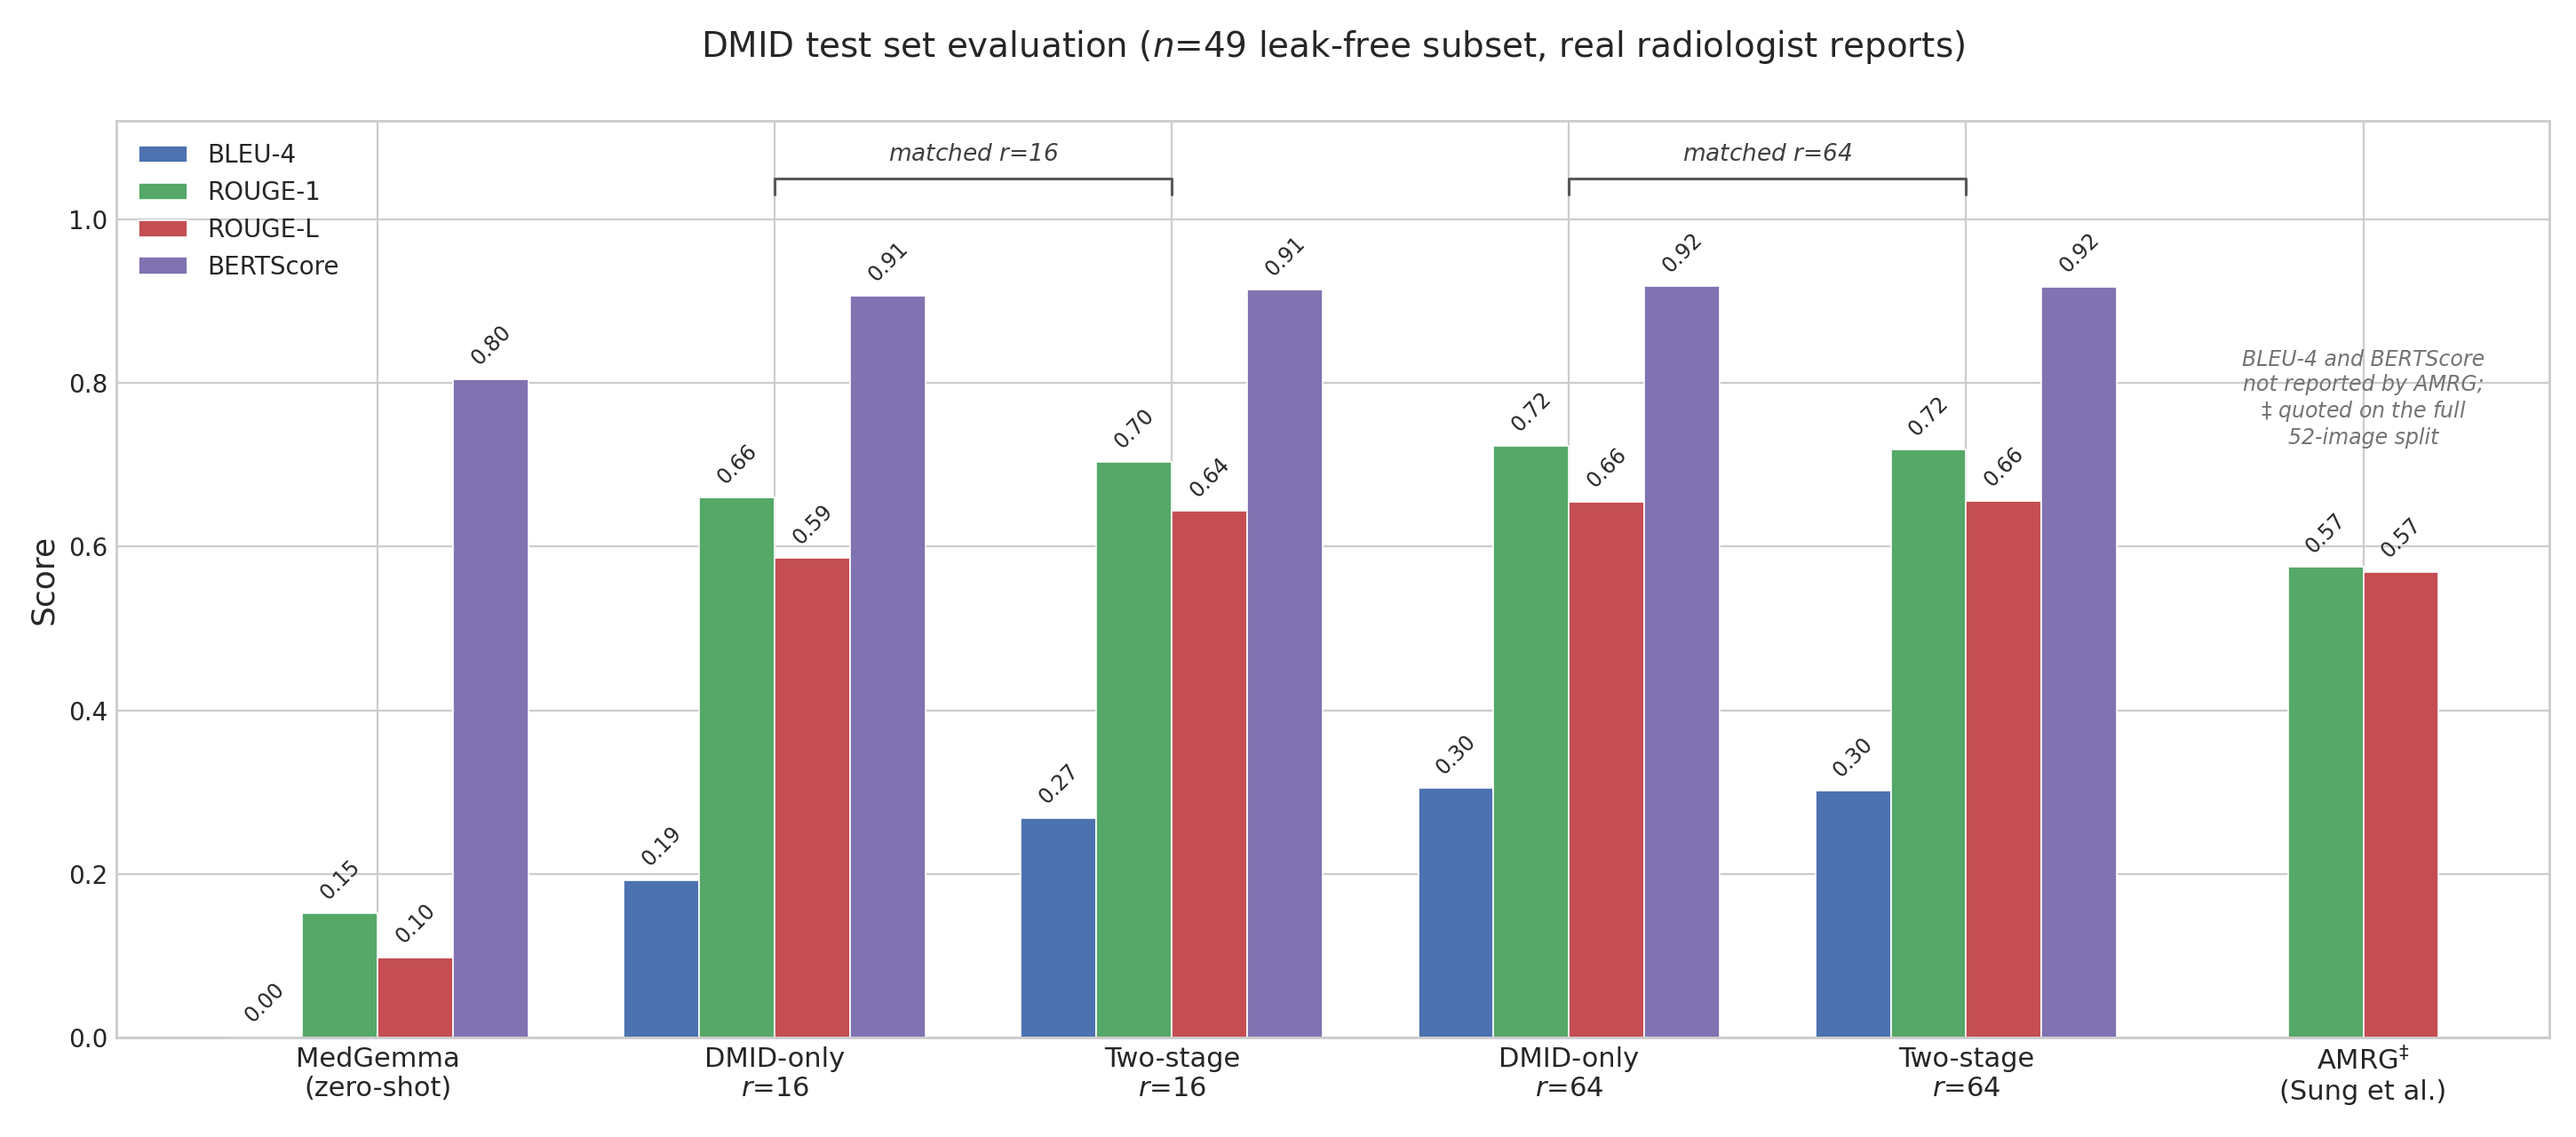
\includegraphics[width=\textwidth]{fig_dmid_ablation.png}
\caption{DMID test set comparison across key methods \revf{on the leak-free subset ($n=49$)}, with the two training schemes shown at matched adapter rank. \revf{The AMRG bars are quoted on the full 52-image split as published and are marked accordingly.} At $r=64$ the two schemes are visually indistinguishable on every metric.}
\label{fig:dmid_bar}
\end{figure}
\subsection*{Clinical Metric Evaluation}

Table~\ref{tab:clinical} presents clinical quality metrics. In this evaluation, the model must predict clinical attributes directly from mammographic images without any BI-RADS input.

\begin{table}[H]
\centering
\caption{Clinical quality metrics on the \revf{leak-free DMID test subset ($n=49$)}, all models at matched adapter rank. Hallucination and omission follow the assertion-level definition of Eq.~(\ref{eq:halluc}); density accuracy is computed on \revf{all 49 cases} rather than on a hand-picked subset. ``Downgraded'' counts reference-suspicious cases (BI-RADS 4--5, $n=22$) that the model assigned to BI-RADS 1--2, the clinically most consequential error. \revf{The three excluded cases are all normal breasts, so the denominators of this table---22 suspicious cases and 40 cases whose reference asserts a finding---are the same as on the full split.} \revf{These are surrogate measures computed against the reference reports, not expert adjudication.}}
\label{tab:clinical}
\begin{adjustbox}{max width=\textwidth}
\begin{tabular}{lcccccccc}
\toprule
& \multicolumn{3}{c}{\textbf{BI-RADS}} & \multicolumn{3}{c}{\textbf{Findings}} & \multicolumn{2}{c}{\textbf{ACR density}} \\
\cmidrule(lr){2-4} \cmidrule(lr){5-7} \cmidrule(lr){8-9}
\textbf{Method} & \textbf{Exact} & $\kappa$ & \textbf{Downgr.} & \textbf{Sens.} & \textbf{Omis.} & \textbf{Halluc.} & \textbf{Acc.} & $\kappa$ \\
\midrule
MedGemma-4B (ZS) & \revf{0.333$^\dagger$} & 0.000 & 0/3$^\dagger$ & 0.300 & 0.700 & 0.000 & \revf{0.176$^\ddagger$} & \revf{$-0.026$} \\
\midrule
DMID-only, $r{=}16$ & \revf{0.327} & \revf{0.126} & 8/22 & \textbf{0.575} & 0.425 & 0.000 & \revf{0.388} & 0.000 \\
Two-stage, $r{=}16$ & \revf{0.286} & \revf{0.080} & 10/22 & 0.525 & 0.475 & 0.000 & \revf{\textbf{0.490}} & \revf{0.108} \\
DMID-only, $r{=}64$ & \revf{0.327} & \revf{0.131} & 7/22 & \textbf{0.675} & 0.325 & 0.000 & \revf{0.449} & 0.000 \\
Two-stage, $r{=}64$ & \revf{0.327} & \revf{\textbf{0.133}} & 7/22 & 0.650 & 0.350 & 0.000 & \revf{0.449} & 0.000 \\
\bottomrule
\end{tabular}
\end{adjustbox}

\footnotesize $^\dagger$\revf{Only 3 of the 49 zero-shot outputs contain a parseable BI-RADS category}; the rate is computed on those 3 and is not comparable with the fine-tuned rows. $^\ddagger$\revf{Computed on the 17 zero-shot outputs stating an ACR category.}
\end{table}

\textbf{The models do not fabricate findings; they omit them.} Under the assertion-level definition of Eq.~(\ref{eq:halluc}) the hallucination rate is $0.000$ for every model, including the zero-shot baseline, while omission ranges from $0.325$ to $0.700$. \rev{A lexical criterion---counting a term as hallucinated when it is absent verbatim from the reference---misclassifies negated mentions such as \emph{``no abnormal soft opacity''} as a hallucinated \emph{opacity}, and produces a spurious hallucination-reduction signal: fine-tuning shortens reports and aligns their vocabulary with the references, which lowers that score without any change in fabrication. On the same generations the two criteria therefore point in opposite clinical directions. Under the assertion-level criterion the dominant error of these models is silence about findings that are present. Of the 49 reference reports, 40 assert at least one finding; the best model (DMID-only, $r=64$) fails to assert a finding in 13 of those 40 cases, that is $32.5\%$ of the cases with a finding and $26.5\%$ of the test set. We state both denominators explicitly because they are not interchangeable.}

\textbf{Synthetic pretraining does not improve finding detection.} At both ranks the DMID-only baseline has the higher sensitivity ($0.575$ vs.\ $0.525$ at $r=16$; $0.675$ vs.\ $0.650$ at $r=64$).

\textbf{The density result does not survive full evaluation.} \rev{A density comparison drawn from 5 hand-picked cases (4/5 vs.\ 1/5) does not hold when every case is scored. Computed on all 49 cases, both $r=64$ models score $0.449$ with $\kappa = 0$: they assign ACR B to every case, and their accuracy is the prevalence of ACR B in the test set, not evidence of density perception. DMID-only at $r=16$ behaves the same way with a different constant, assigning ACR C to every case for an accuracy of $0.388$. The one configuration with non-trivial density agreement is two-stage at $r=16$ ($\kappa = 0.108$), which is also the configuration with the worst BI-RADS agreement in the table. Occasional per-seed exceptions to $\kappa \approx 0$ occur but do not reproduce across initialisations.}

Generated reports average \revf{$37.9$} words (two-stage, $r=64$) and \revf{$39.1$} words (DMID-only, $r=64$) against \revf{$44.2$} words for the reference reports, compared with \revf{$118.6$} words for the zero-shot baseline; fine-tuning calibrates report length, and the two schemes are indistinguishable in this respect as well.

\subsection*{BI-RADS Distribution and Per-Category Analysis}

\revf{The leak-free DMID test subset exhibits the following BI-RADS distribution: BI-RADS 1 (16.3\%, $n=8$), BI-RADS 2 (14.3\%, $n=7$), BI-RADS 3 (24.5\%, $n=12$), BI-RADS 4 (30.6\%, $n=15$), and BI-RADS 5 (14.3\%, $n=7$). Breast density distribution spans ACR A (6.1\%), ACR B (44.9\%), ACR C (38.8\%), and ACR D (10.2\%).}

\revf{The predominance of ACR B density in the test subset (44.9\%) explains the density accuracy of both $r=64$ models without any appeal to density perception. Both assign ACR B to all 49 cases, so their accuracy of $0.449$ is exactly the prevalence of ACR B and their agreement with the reference is $\kappa = 0$.} VinDr-Mammo, on which Stage~1 is built, is likewise dominated by ACR B, so the constant prediction is consistent with inheriting the majority class of the pretraining distribution rather than with transferring density knowledge.

The overall BI-RADS accuracy of \revf{$0.327$} masks substantial variation across categories, and the variation runs in the clinically unfavourable direction. Normal cases (BI-RADS 1--2) are identified far more reliably than suspicious ones: of the 22 reference-suspicious cases, 7 are assigned to BI-RADS 1--2 by both $r=64$ models. Agreement beyond chance is low for every model in this study (\revf{$\kappa$ between $0.08$ and $0.13$}). This is consistent with the clinical difficulty of distinguishing subtle malignant features~\cite{sechopoulos2021artificial}. \rev{Two properties of the setup are plausible contributors, which we name as hypotheses rather than as measured causes: each image is scored in isolation, so the cross-view correspondence a radiologist uses between the CC and MLO projections is unavailable to the model, and the encoder input resolution is far below the native one. Both are taken up in Limitations.} \rev{Low agreement} is the principal obstacle to any clinical use of these outputs; class-balanced training or BI-RADS-specific loss weighting remain plausible directions, but the gap is large enough that we do not present the current accuracy as adequate for assistance in reporting.

\rev{Fine-tuning does change output behaviour substantially, but in a narrower way than fluency scores suggest. In the zero-shot setting MedGemma-4B~\cite{lin2024medgemma} produces verbose, unstructured responses averaging $118.6$ words, only 3 of which contain a parseable BI-RADS category, whereas every fine-tuned model produces a BI-RADS category and an ACR category in all 49 cases and averages $36$--$39$ words against $44.2$ for the references. What fine-tuning delivers is structural conformity and length calibration. It does not reduce fabrication, because under an assertion-level criterion no model fabricates findings at any stage; and it does not improve category agreement beyond $\kappa \approx 0.13$.}

\subsection*{Data Efficiency Analysis}

Figure~\ref{fig:efficiency} presents the data efficiency analysis across varying amounts of real training data; the underlying numbers are given in Supplementary Table~S2.


Within this experiment the two-stage curve lies above the DMID-only curve at every data volume. \rev{The differences} on which such a conclusion would rest are smaller than the run-to-run variability we measured elsewhere in this study: the gap between two-stage at $N=200$ ($0.599$) and DMID-only at $N=407$ ($0.615$) is $0.0155$, and the margin over the AMRG benchmark at $N=100$ is $0.001$, against a between-initialisation standard deviation of \revf{$0.034$--$0.045$} ROUGE-L for a fixed configuration. A single initialisation per point cannot separate these differences from initialisation noise. \rev{No data-efficiency claim is drawn from this experiment.}


\begin{figure}[H]
\centering
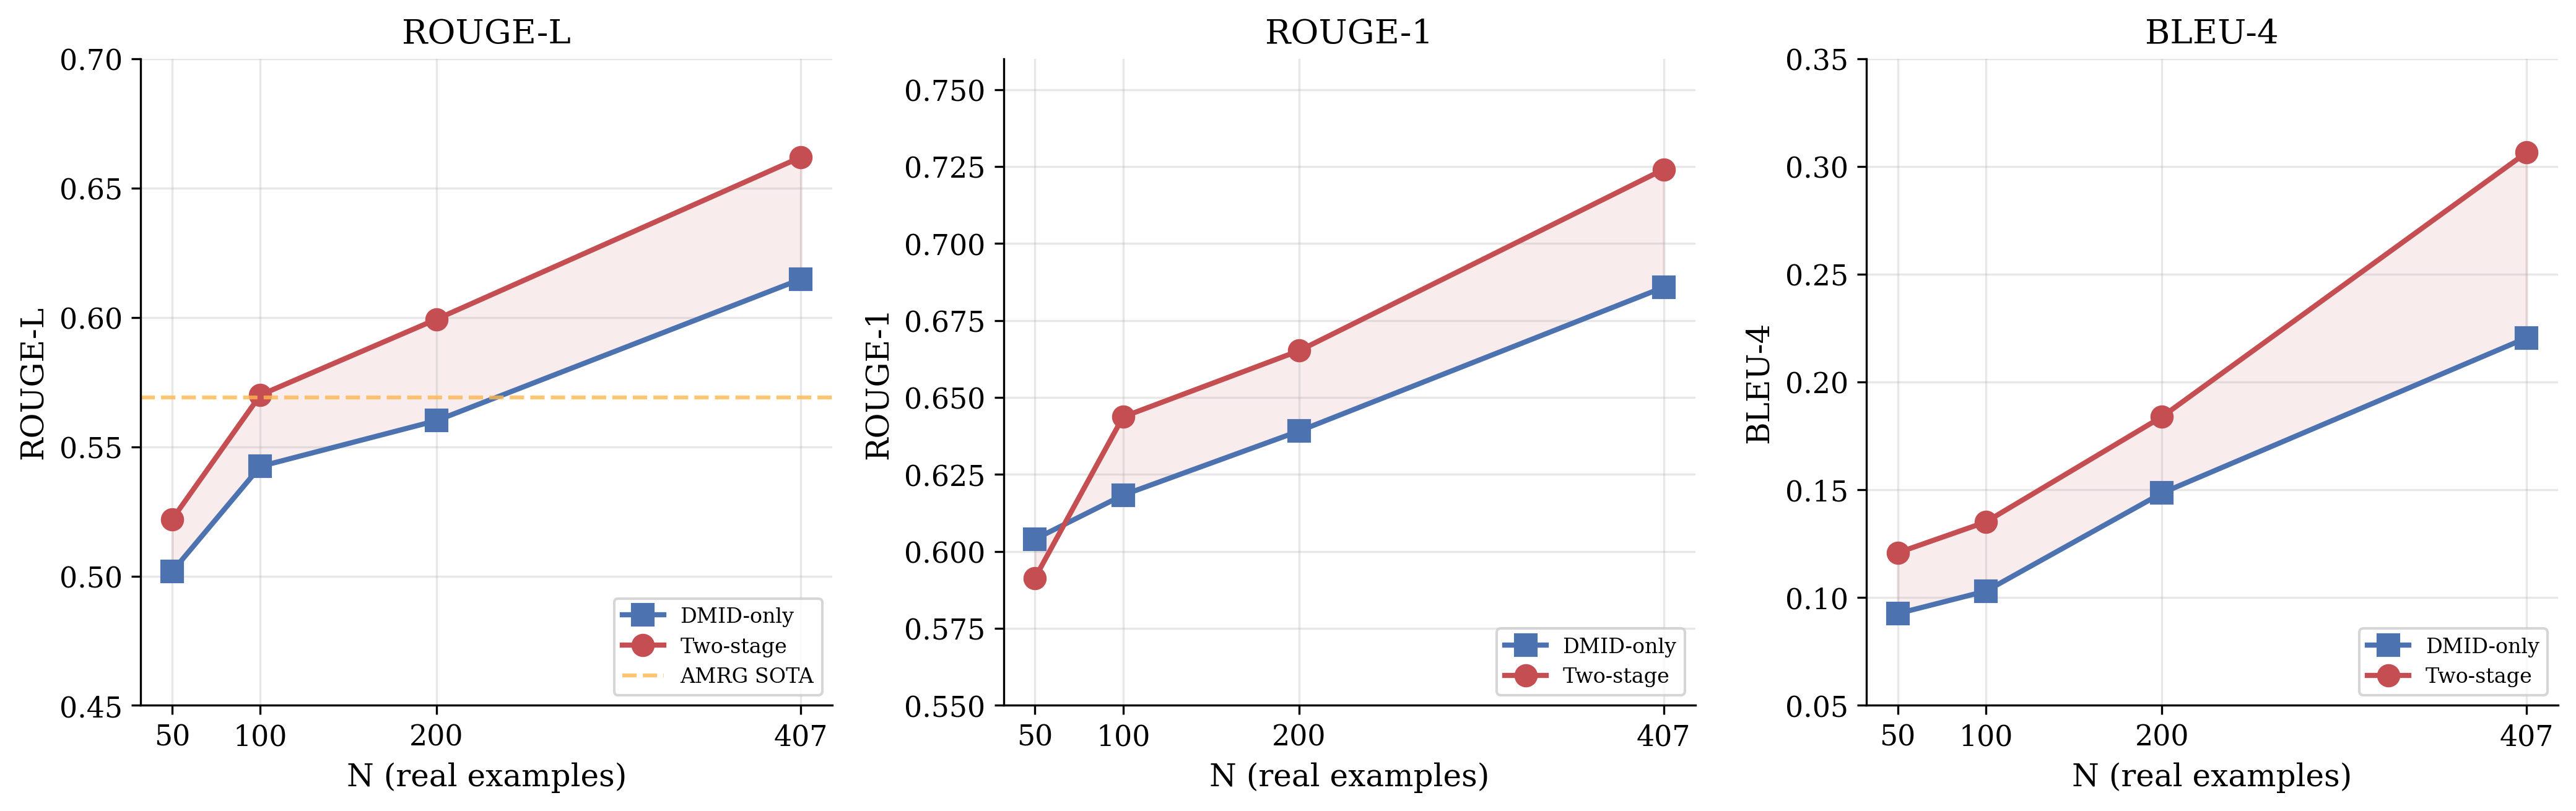
\includegraphics[width=\textwidth]{fig_data_efficiency.png}
\caption{Data efficiency analysis under the protocol of Supplementary Table~S2 ($r=16$, one initialisation per point). Error bars are unavailable because per-sample generations were not retained; the separation between the curves is smaller than the between-initialisation variability measured for a fixed configuration elsewhere in this study, and no data-efficiency claim is drawn from it.}
\label{fig:efficiency}
\end{figure}

\subsection*{Training Dynamics}

Figure~\ref{fig:curves} compares training dynamics. The two-stage model starts with lower initial training loss (3.33 vs. 4.00) and achieves lower best validation loss (0.655 vs. 0.669), which is consistent with synthetic pretraining providing a domain-adapted initialisation~\cite{pan2010transfer}. The lower starting loss is expected and robust: the Stage~1 adapter has already seen mammography report vocabulary and formatting. The difference in \emph{best} validation loss is a single-run difference of $0.014$ and should not be read as evidence of a better final model, since it does not translate into a difference in test-set output at matched capacity (Table~\ref{tab:equalcap}).


\begin{figure}[H]
\centering
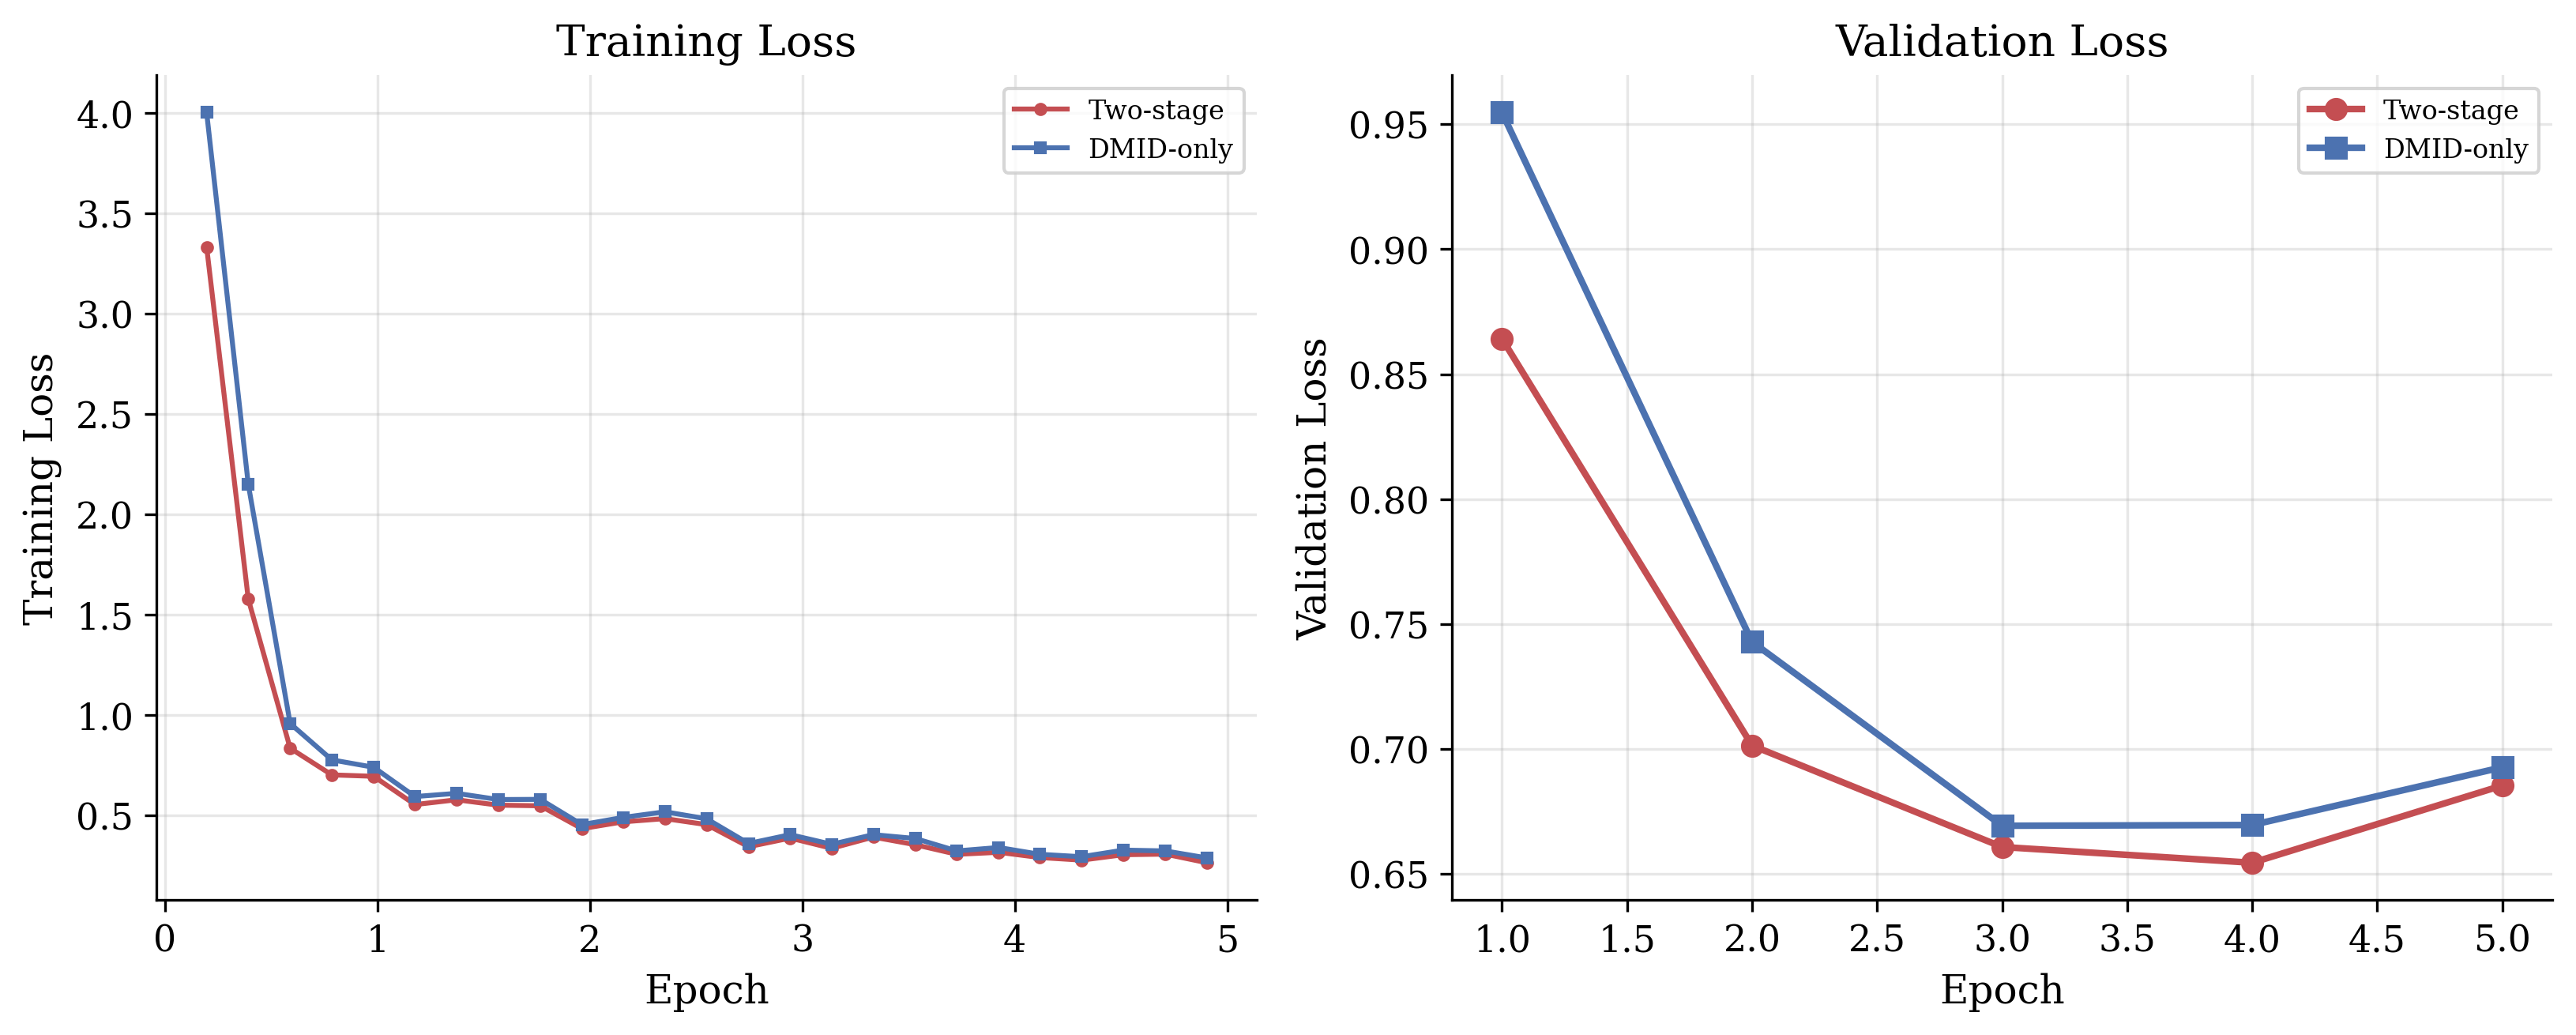
\includegraphics[width=\textwidth]{fig_training_curves.png}
\caption{Training dynamics. Two-stage benefits from lower initial loss and achieves lower best validation loss (0.655 vs. 0.669).}
\label{fig:curves}
\end{figure}

\subsection*{Qualitative Analysis}

Table~\ref{tab:qualitative} presents representative generated reports with colour-coded clinical term evaluation: \textcolor{correct}{correct terms (blue)}, \textcolor{incorrect}{incorrect terms (red)}, and \textcolor{hallucinated}{findings present in the reference but omitted from the generated report (green)}. \rev{The third category marks omission rather than fabrication, because no fabricated finding occurs in any generation under the criterion of Eq.~(\ref{eq:halluc}), whereas omission is the dominant error.} Both branches are shown at $r=64$, the matched-capacity comparison. All three examples are drawn from the 49 test cases whose reference report does not appear in the training split.

\begin{table}[H]
\centering
\caption{Qualitative comparison of generated mammography reports at matched adapter rank ($r=64$). Clinical terms: \textcolor{correct}{correct (blue)}, \textcolor{incorrect}{incorrect (red)}, \textcolor{hallucinated}{omitted from the generation (green)}.}
\label{tab:qualitative}
\small
\begin{tabularx}{\textwidth}{p{1.8cm}p{1.4cm}X}
\toprule
\textbf{Image} & \textbf{Method} & \textbf{Generated Report} \\
\midrule
\multicolumn{3}{l}{\textbf{Example 1: Img510 --- Normal breast (BI-RADS 1) --- both schemes correct and identical}} \\
\midrule
\multirow{3}{*}{\includegraphics[width=1.6cm]{mammo_510.png}}
& \textbf{GT} & BC: \textcolor{correct}{fibro fatty and glandular (ACR B)}. F: \textcolor{correct}{no abnormal soft opacity or microcalcification}. \textcolor{correct}{Skin, nipple and pectoral muscle appear normal}. \textcolor{correct}{No significant axillary nodes}. \textcolor{correct}{BIRADS: 1} \\
\addlinespace
& \textbf{Two-stage} & BC: \textcolor{correct}{fibro fatty and glandular (ACR B)}. F: \textcolor{correct}{No abnormal soft opacity or microcalcification}. \textcolor{correct}{Skin, nipple and pectoral muscle appear normal}. \textcolor{correct}{No significant axillary adenopathy}. \textcolor{correct}{BIRADS: 1} \\
\addlinespace
& \textbf{DMID-only} & \emph{token-identical to the two-stage output above} \\
\midrule
\multicolumn{3}{l}{\textbf{Example 2: Img501 --- Malignant lesion (BI-RADS 5) --- both schemes fail identically}} \\
\midrule
\multirow{3}{*}{\includegraphics[width=1.6cm]{mammo_501.png}}
& \textbf{GT} & BC: \textcolor{correct}{dense glandular (ACR D)}. F: \textcolor{hallucinated}{a large well defined lobulated soft opacity with foci of microcalcifications in the posterior aspect of the outer quadrant, suggesting malignant lesion}. \textcolor{hallucinated}{BIRADS: 5} \\
\addlinespace
& \textbf{Two-stage} & BC: \textcolor{incorrect}{fibro fatty and glandular (ACR B)}. F: \textcolor{incorrect}{No abnormal soft opacity or microcalcification seen}. \textcolor{correct}{Skin and nipple appear normal}. \textcolor{incorrect}{BIRADS: 1} \\
\addlinespace
& \textbf{DMID-only} & \emph{token-identical to the two-stage output above} \\
\midrule
\multicolumn{3}{l}{\textbf{Example 3: Img463 --- Normal breast (BI-RADS 1) --- constant density prediction}} \\
\midrule
\multirow{3}{*}{\includegraphics[width=1.6cm]{mammo_463_clean.png}}
& \textbf{GT} & BC: \textcolor{correct}{fibro fatty and glandular (ACR C)}. F: \textcolor{correct}{No abnormal soft opacity or microcalcifications}. \textcolor{correct}{No significant axillary adenopathy}. \textcolor{correct}{BIRADS: 1} \\
\addlinespace
& \textbf{Two-stage} & BC: \textcolor{incorrect}{fibro fatty and glandular (ACR B)}. F: \textcolor{correct}{No abnormal soft opacity or microcalcification}. \textcolor{correct}{No significant axillary adenopathy}. \textcolor{correct}{BIRADS: 1} \\
\addlinespace
& \textbf{DMID-only} & BC: \textcolor{incorrect}{fibro fatty and glandular (ACR B)}. F: \textcolor{correct}{No abnormal soft opacity or microcalcification}. \textcolor{correct}{BIRADS: 1} \\
\bottomrule
\end{tabularx}
\end{table}

The three examples were selected to illustrate the range of behaviour rather than to favour either scheme, and in all three the two training schemes are difficult to tell apart. Example~1 is a normal breast reported correctly, where the two branches emit token-identical text. Example~2 is the clinically consequential failure mode quantified in Table~\ref{tab:clinical}: the reference describes a large lobulated opacity with microcalcifications and assigns BI-RADS 5, and both models state that no abnormality is seen and assign BI-RADS 1. Note that this is an omission, not a fabrication---the model is silent about a lesion that is present---and that the two schemes fail in exactly the same way. Example~3 shows the constant density prediction: the reference states ACR C and both models state ACR B, as they do for \revf{all 49 test cases}.

\subsection*{LoRA Hyperparameter Ablation}

Table~\ref{tab:lora} presents LoRA~\cite{hu2022lora} rank and scaling factor ablation for Stage~2, with Stage~1 held constant at $r=16, \alpha=32$.

\begin{table}[H]
\centering
\caption{LoRA hyperparameter ablation. Stage~1 uses $r=16, \alpha=32$; Stage~2 varies. \revf{All rows use the merging mechanism of Eq.~(\ref{eq:merge}) with identical hyperparameters, so that they differ only in $r$ and $\alpha$.} Configurations are ranked by ROUGE-L on the \emph{validation} split ($n=51$); test values are reported for completeness but were not used for selection. \revf{The test column of this table alone is computed on the full 52-image split: per-sample generations were not retained for five of the seven configurations, so the leak-free recomputation used in Tables~\ref{tab:dmid}--\ref{tab:clinical} is not available here. The validation split is unaffected by the test-split leakage.} Rows are ordered by validation ROUGE-L.}
\label{tab:lora}
\begin{adjustbox}{max width=\textwidth}
\begin{tabular}{ccccccccc}
\toprule
& & & \multicolumn{5}{c}{\textbf{Test split} ($n=52$)} & \textbf{Val.} \\
\cmidrule(lr){4-8} \cmidrule(lr){9-9}
$r$ & $\alpha$ & \textbf{Params} & \textbf{BLEU-4} & \textbf{ROUGE-1} & \textbf{ROUGE-L} & \textbf{METEOR} & \textbf{CIDEr} & \textbf{ROUGE-L} \\
\midrule
64 & 64 & 131.1M & 0.312 & 0.734 & 0.671 & 0.685 & 0.729 & \textbf{0.5915} \\
32 & 64 & 65.5M & 0.296 & 0.726 & 0.661 & 0.672 & 0.623 & 0.5913 \\
16 & 32 & 32.8M & 0.285 & 0.716 & 0.648 & 0.656 & 0.591 & 0.5795 \\
32 & 32 & 65.5M & 0.290 & 0.714 & 0.648 & 0.656 & 0.646 & 0.5776 \\
64 & 128 & 131.1M & 0.268 & 0.728 & 0.666 & 0.671 & 0.687 & 0.5766 \\
8 & 32 & 16.4M & 0.289 & 0.721 & 0.654 & 0.660 & 0.613 & 0.5757 \\
8 & 16 & 16.4M & 0.268 & 0.700 & 0.631 & 0.633 & 0.527 & 0.5502 \\
\bottomrule
\end{tabular}
\end{adjustbox}
\end{table}

\textbf{Capacity matters; the specific optimum does not.} Adapter rank has a clear effect at the low end: moving from $r=8,\alpha=16$ to $r=32$ raises validation ROUGE-L from $0.5502$ to $0.5776$--$0.5913$. Above $r=32$ the curve is flat. The separation between the top two configurations is $0.0002$ ROUGE-L on validation, against a between-initialisation standard deviation of \revf{$0.011$--$0.033$} for fixed configurations at these ranks (\revf{$0.011$--$0.045$} across the full grid). \rev{We therefore do not identify $r=64,\alpha=64$ as an optimum.} Configurations from $r=32$ upward are statistically indistinguishable, and $r=32,\alpha=64$ is preferable in practice since it reaches the same quality with half the trainable parameters. The middle of the ranking is also unstable: $r=64,\alpha=128$ places second on test but fifth on validation.

\rev{\textbf{Capacity, not the two-stage scheme, drives the gains.} A table of two-stage configurations that all exceed the AMRG benchmark does not by itself implicate the two-stage paradigm, because the comparison contains no equal-capacity DMID-only baseline. When one is trained, the DMID-only baseline improves with rank in the same way ($0.6161 \rightarrow 0.6443 \rightarrow 0.6394$ ROUGE-L for $r=16, 32, 64$, averaged over three initialisations). The gain from raising the rank from $16$ to $32$ is $0.028$ ROUGE-L, larger than the difference between the two training schemes at any fixed rank anywhere in the grid below (at most $0.011$).}


\subsection*{Equivalence Analysis}

The comparisons above are single-run comparisons. To test whether synthetic pretraining has an effect that survives replication, we retrained both branches across a grid of \rev{36 Stage~2 training runs: 27 two-stage runs (three Stage~1 corpus sizes---369, 800 and 1444 synthetic pairs---by three adapter configurations, $r=16,\alpha=32$; $r=32,\alpha=64$; $r=64,\alpha=64$, by three random initialisations, seeds 42, 43 and 44), plus 9 DMID-only baselines (three configurations by three initialisations), which are shared across the three corpus-size rows of a column because a DMID-only run has no Stage~1 and therefore does not depend on the corpus. The 27 two-stage runs rest on 9 Stage~1 pretraining runs, one per corpus size and initialisation. A further three two-stage runs at $r=16$ on the original Stage~1 corpus provide the preregistered contrast reported at the end of this subsection.} \rev{The Stage~1 corpus was regenerated for the grid} with the language contamination removed---it contains no Cyrillic text---and rebalanced between VinDr-Mammo and CBIS-DDSM, so that a null result cannot be attributed to the defects of the original corpus.

Rather than testing for a difference, we test for equivalence, since the question is whether the two schemes can be treated as interchangeable. We use two one-sided tests (TOST) on $\Delta = \text{ROUGE-L}(\text{two-stage}) - \text{ROUGE-L}(\text{DMID-only})$ with an equivalence margin $\Delta_{\text{eq}} = 0.02$ ROUGE-L, fixed before the runs were executed, and 90\% confidence intervals. A cell is declared \emph{equivalent} when the interval lies entirely within $\pm\Delta_{\text{eq}}$, \emph{superior} when it lies entirely above $+\Delta_{\text{eq}}$, and \emph{inconclusive} otherwise. Table~\ref{tab:tost} reports the nine cells.

\begin{table}[H]
\centering
\caption{Equivalence testing of the two training schemes across Stage~1 corpus size and adapter capacity, \revf{on the leak-free test subset ($n=49$)}. \revf{Each cell aggregates three initialisations per branch; the DMID-only runs are shared across the three corpus-size rows of a column.} $\Delta$ is two-stage minus DMID-only in ROUGE-L; intervals are 90\% confidence intervals; the equivalence margin is $\Delta_{\text{eq}} = 0.02$. \revf{The margin was fixed before any run was executed and is applied to the leak-free subset unchanged.} \textbf{E} = equivalent, \textbf{I} = inconclusive; no cell is superior.}
\label{tab:tost}
\begin{adjustbox}{max width=\textwidth}
\begin{tabular}{lcccccc}
\toprule
& \multicolumn{2}{c}{$r=16, \alpha=32$} & \multicolumn{2}{c}{$r=32, \alpha=64$} & \multicolumn{2}{c}{$r=64, \alpha=64$} \\
\cmidrule(lr){2-3} \cmidrule(lr){4-5} \cmidrule(lr){6-7}
\textbf{Stage~1 pairs} & $\Delta$ & \textbf{90\% CI} & $\Delta$ & \textbf{90\% CI} & $\Delta$ & \textbf{90\% CI} \\
\midrule
\revf{369} & \revf{$+0.0032$} & \revf{$[-0.0163, +0.0227]$ \textbf{I}} & \revf{$-0.0077$} & \revf{$[-0.0232, +0.0078]$ \textbf{I}} & \revf{$+0.0093$} & \revf{$[-0.0284, +0.0469]$ \textbf{I}} \\
\revf{800} & \revf{$+0.0034$} & \revf{$[-0.0036, +0.0103]$ \textbf{E}} & \revf{$-0.0067$} & \revf{$[-0.0319, +0.0185]$ \textbf{I}} & \revf{$-0.0009$} & \revf{$[-0.0028, +0.0011]$ \textbf{E}} \\
\revf{1444} & \revf{$+0.0027$} & \revf{$[-0.0081, +0.0135]$ \textbf{E}} & \revf{$-0.0024$} & \revf{$[-0.0203, +0.0156]$ \textbf{I}} & \revf{$+0.0111$} & \revf{$[-0.0075, +0.0297]$ \textbf{I}} \\
\bottomrule
\end{tabular}
\end{adjustbox}
\end{table}

\rev{Three cells are equivalent, six are inconclusive, and none shows superiority. The largest absolute difference anywhere in the grid is $0.0111$, roughly half the equivalence margin; the inconclusive verdicts are caused by the width of the confidence intervals at three runs per cell, not by the size of the effect. We therefore claim equivalence only for the three cells whose interval lies entirely within the margin, and read the remaining six as absence of evidence for superiority rather than as demonstrated equivalence.}

Three observations follow. First, there is no dose response: \revf{at $r=16$ the difference is $+0.0032$, $+0.0034$ and $+0.0027$} as the synthetic corpus grows fourfold, so the null result cannot be explained by an insufficient quantity of synthetic data. Second, the sign of the difference is set by adapter rank rather than by the training scheme---\revf{all three cells of the $r=32$ column are negative and all three of the $r=16$ column positive, while the $r=64$ column changes sign}---which is the signature of noise rather than of an effect. Third, initialisation variance dominates: the between-seed standard deviation within a single branch is \revf{$0.011$--$0.045$} ROUGE-L, more than an order of magnitude larger than the $\sim\!0.005$ difference between branches, and seed 44 underperformed in every cell of both branches, which identifies it as an initialisation effect rather than a property of either training scheme.

We state the status of this analysis explicitly. The preregistered contrast is the single comparison at $r=16$ on the original Stage~1 corpus; the grid over corpus size on the regenerated corpus is \emph{exploratory} and was not preregistered. The equivalence margin and the decision rule, however, were fixed in advance for all cells. \rev{On the leak-free subset the preregistered contrast gives $\Delta = -0.0033$ with 90\% CI $[-0.0143, +0.0077]$, an equivalent verdict. We also note that the main conclusion does not depend on the defects of the original corpus: every cell of the grid was trained on the regenerated Stage~1 corpus, which contains no Cyrillic text and therefore no language contamination.}

\subsection*{Retrieval Ablation}

We tested the contribution of the BI-RADS retrieval module directly, by evaluating the final two-stage model ($r=64$) on the \revf{leak-free DMID test subset} with and without the retrieved passage in the prompt, holding everything else fixed. Retrieval decreases every one of the six text metrics and CIDEr. \revf{The decrease is significant for BLEU-4 ($\Delta = -0.0434$, 95\% CI $[-0.0735, -0.0180]$, $p=0.0028$) and ROUGE-2 ($\Delta = -0.0412$, 95\% CI $[-0.0818, -0.0047]$, $p=0.0392$); for ROUGE-L the change is $-0.0158$ ($p=0.33$) and is not significant. CIDEr falls from $0.649$ to $0.450$.}

This is a negative result and we report it as one. Retrieving a passage of the BI-RADS Atlas into the prompt does not improve generated reports and measurably degrades some of them, plausibly because the retrieved text introduces vocabulary that does not appear in the terse DMID reference reports. The models reported in Tables~\ref{tab:dmid}--\ref{tab:lora} therefore do not use retrieval at inference, \rev{and the retrieval module is reported as an ablated component rather than as part of the framework}.

%% ─────────────────────────────────────────────────────────────────
\section*{Discussion}
%% ─────────────────────────────────────────────────────────────────

\textbf{Synthetic pretraining does not improve final report quality at matched capacity.} The central finding of this analysis is negative. \rev{Across 36 training runs spanning three synthetic corpus sizes, three adapter capacities and three initialisations, no configuration shows the two-stage scheme to be superior, three of nine cells are statistically equivalent, and the largest difference observed anywhere is half the prespecified equivalence margin.}

\rev{An unmatched comparison---the DMID-only baseline at $r=16$ against the two-stage model at $r=64$, the two branches evaluated under different prompts, connected by different transfer mechanisms and each trained from a single initialisation---shows an apparent advantage of $+0.070$ ROUGE-L for two-stage training. Adapter rank alone accounts for it: raising the DMID-only baseline from $r=16$ to $r=64$ with nothing else changed gains $+0.069$. The gap that remains between the branches at the matched rank $r=16$ is $+0.058$, and three further factors contribute to it, each measured separately on the same models: an evaluation prompt that costs the DMID-only baseline four times as much as the two-stage model ($0.0149$ vs.\ $0.0034$ ROUGE-L); a difference in the Stage~1 $\rightarrow$ Stage~2 transfer mechanism, worth $0.012$ ROUGE-L between the continuation and merging variants of the two-stage model at $r=16$; and a single random initialisation, against a between-initialisation spread of up to $0.08$ ROUGE-L at this rank, under which the $r=16$ difference falls to $+0.003$ on replication. None of the four factors is a property of synthetic pretraining.} What synthetic pretraining does provide is a better starting point---lower initial training loss (3.33 vs.\ 4.00), consistent with domain-adapted initialisation~\cite{bengio2012deep, pan2010transfer}---but this advantage is exhausted during Stage~2 and leaves no measurable trace in the final model.

We report this as a robust negative result rather than as a failed experiment. The regenerated Stage~1 corpus is four times larger than the original and free of the language contamination we identified, so the null result cannot be attributed to insufficient or defective synthetic data; and the effect is absent at every capacity we tested rather than at one operating point.

\textbf{Comprehensive SOTA comparison.} \rev{At $r=64$ our fine-tuned models outperform all eight evaluated baseline methods, spanning four architectural paradigms, on every text metric and under either training scheme; at $r=16$ the DMID-only baseline falls below the CLIP+GPT2 pipeline on BLEU-4, ROUGE-1 and ROUGE-L. Against AMRG~\cite{sung2025} (the previous SOTA), the two-stage model at $r=64$ improves ROUGE-L by $15.3\%$, METEOR by $8.4\%$ and CIDEr by $11.6\%$, with the caveat that AMRG was evaluated on a different split of DMID and with a different category-extraction rule, was not re-run under our protocol, and is therefore not measured on the same images.} Notably, pipeline approaches (CLIP~\cite{radford2021clip}+GPT2~\cite{radford2019gpt2}) achieve competitive ROUGE-L (0.613) but markedly lower CIDEr (0.078), suggesting that end-to-end VLM fine-tuning produces more fluent and better-calibrated reports\revf{; those two rows are quoted on the full 52-image split (Table~\ref{tab:dmid})}.


\textbf{Clinical quality does not follow textual quality.} Fine-tuning produces reports that are structurally well formed, correctly sized and lexically close to radiologist reports, and none of this translates into clinical reliability. Agreement with the reference BI-RADS category is low for every model in this study (\revf{$\kappa$ between $0.08$ and $0.13$}), density prediction is constant at the majority class for the $r=64$ models ($\kappa = 0$), and of 22 reference-suspicious cases 7 are assigned to BI-RADS 1--2. Under an assertion-level criterion no model fabricates findings; the characteristic failure is silence about findings that are present, affecting between a third and a half of the cases in which the reference asserts one.

The clearest evidence that fluency and reliability can move in opposite directions comes from within a single model rather than from comparing different sources. At $r=16$ the two-stage model beats the DMID-only baseline on every text metric, by $+0.058$ ROUGE-L at $p=0.0001$. At that same operating point it is clinically worse: BI-RADS agreement falls (\revf{$\kappa$ $0.080$ vs.\ $0.126$}), finding sensitivity falls ($0.525$ vs.\ $0.575$), and it downgrades 10 of 22 suspicious cases to benign against 8 for the baseline. A reviewer or reader given only the text metrics at this operating point would select the clinically inferior model. This is a concrete argument against selecting mammography report generators on $n$-gram overlap, and it is measured here within one architecture and one dataset, so it cannot be attributed to differences between sources. The attention mechanisms explored in our prior work~\cite{esen2025multitask} and Grad-CAM~\cite{selvaraju2017gradcam} interpretability~\cite{esen2025rl} provide complementary approaches to building clinician trust, but the gap identified here is one of diagnostic accuracy, not of explanation.

\textbf{Architectural paradigm comparison.} Our evaluation spans four distinct architectural paradigms. Zero-shot VLMs (LLaVA~\cite{liu2024llava}, Qwen~\cite{wang2024qwen2vl}, MedGemma~\cite{lin2024medgemma}) uniformly perform poorly on mammography, with ROUGE-L below 0.15, indicating that general-purpose VLM pretraining does not transfer to specialised mammographic reporting. Pipeline approaches (CLIP+GPT2) achieve surprisingly competitive results after fine-tuning (ROUGE-L: 0.571--0.613). However, end-to-end VLM fine-tuning with our two-stage approach consistently outperforms pipeline methods across all metrics, particularly CIDEr (\revf{0.649}), indicating superior clinical coherence.

\textbf{Comparison with AMRG methodology.} Both our approach and AMRG~\cite{sung2025} fine-tune MedGemma-4B~\cite{lin2024medgemma} with LoRA~\cite{hu2022lora} on DMID. \rev{Three differences could in principle explain our higher text scores, and only one of them survives measurement.} Adapter capacity is the substantive one: AMRG uses $r=32,\alpha=16$, and we find that scaling factor to be low relative to rank, whereas the $\alpha \geq r$ configurations we tested cluster at the top of the ranking. \rev{The second candidate---that two-stage pretraining supplies an initialisation absent from direct fine-tuning---is not supported by our own equal-capacity comparison, since our DMID-only baseline, which is also direct fine-tuning, matches the two-stage model. The third, that synthetic augmentation and retrieval contribute to robustness, is contradicted by the retrieval ablation. We also note that AMRG's BI-RADS accuracy of $0.558$ exceeds every model in this study by roughly $0.23$, and that increasing adapter capacity does not close that gap: raising the rank of the DMID-only baseline from $r=16$ to $r=64$ gains $0.069$ ROUGE-L while leaving its BI-RADS accuracy unchanged at $0.327$.} Whatever produces AMRG's clinical accuracy is not adapter capacity, and identifying it is more valuable than the text-metric margin we report.

\textbf{LoRA configuration analysis.} Our ablation across seven configurations shows a capacity effect that saturates. Validation ROUGE-L rises from $0.550$ at $r=8,\alpha=16$ to $0.578$--$0.591$ at $r=32$ and does not improve further at $r=64$; the top two configurations differ by $0.0002$, well inside run-to-run noise. We therefore report a practical recommendation rather than an optimum: use $r \geq 32$ with $\alpha \geq r$, and prefer $r=32,\alpha=64$ for its lower cost at equal quality. \rev{The capacity effect is not attributable to the two-stage paradigm, since the DMID-only baseline shows the same rank dependence.}

\textbf{Context within broader research.} Our results complement recent clinical AI deployment studies~\cite{dembrower2020effect, salim2020external, aboutalib2018deep}, suggesting that automated report generation could reduce radiologist workload while maintaining diagnostic quality. The detection capabilities demonstrated by Shen et al.~\cite{shen2019deep} and Ribli et al.~\cite{ribli2018detecting} in Scientific Reports, along with the feature extraction approaches by Aitimov et al.~\cite{aitimov2025feature} from Kazakhstan, highlight the growing maturity of deep learning for mammography analysis. Modern architectures including ResNet~\cite{he2016deep}, DenseNet~\cite{huang2017densely}, transformers~\cite{vaswani2017attention}, and Vision Transformers~\cite{dosovitskiy2021vit} have been foundational to this progress. Unlike chest X-ray report generation which benefits from large-scale datasets~\cite{johnson2019mimiccxr}, mammography faces severe data scarcity, making our synthetic-to-real approach particularly valuable.

\textbf{Retrieval.} Retrieval degrades generation at both stages: it lowered NLP metrics in Stage~1, and the controlled ablation on the final model shows significant decreases in BLEU-4 and ROUGE-2 with no metric improved. We therefore present the BI-RADS retrieval module as a component that we implemented and tested and that did not work for this task, rather than as a contribution. A plausible explanation is a register mismatch---Atlas passages are discursive while DMID reports are terse---which suggests that retrieval for report generation should supply structured constraints rather than prose. Entity-level evaluation such as RadGraph F1 would measure this better than $n$-gram overlap.

\textbf{Future work.} The most informative next step suggested by our results is not further scaling of synthetic data---which we have shown does not help---but an investigation of why BI-RADS agreement remains near chance for every model while text similarity is high. \rev{Two candidate causes are testable and untested here: the loss of fine detail at the encoder input resolution, which would require a backbone accepting native-resolution crops or a detector front-end that supplies them, and the absence of cross-view reasoning, which would require view pairing that DMID does not publish. We state both as hypotheses; neither is measured in this study.} Multi-view integration; BI-RADS-guided constrained decoding; extension to other low-resource medical imaging domains; formal radiologist evaluation; reinforcement learning from human feedback (RLHF) building on our prior RL work~\cite{esen2025rl}.

%
\section*{Limitations}

\textbf{Data.} DMID is the only public mammography dataset with paired free-text reports, so the benchmark, the training data and the evaluation all rest on a single source of 225 cases, \revf{and the primary test set contains 49 images}. Every quantity reported here inherits that limitation, and none of our conclusions has been replicated on an independent paired dataset. \rev{Every conclusion of this paper---the equivalence result, the omission-dominant error profile, the divergence between textual and clinical quality---is therefore qualified as single-source: it describes what these models do on DMID, and its generality to other mammography collections is untested.}

\textbf{Split.} The split is image-level rather than patient-level, because the image-to-patient mapping is not published. Three of the 52 test images have a reference report that also occurs in the training split; \revf{we exclude them and report all results on the remaining 49, with the full 52-image split retained as a sensitivity analysis. The two agree.}

\textbf{Clinical accuracy.} BI-RADS agreement is near chance (\revf{$\kappa \leq 0.14$}) for every model we trained, and 7 of 22 suspicious cases are downgraded to BI-RADS 1--2. \revf{These are surrogate measures computed against the reference reports rather than expert judgements.} These outputs are not suitable for clinical use in their present form, and we make no claim that they are. One plausible contributing cause is input resolution: the SigLIP encoder~\cite{zoph2020siglip} operates at $896$ px against native mammograms of $3500$--$4500$ px, so microcalcifications may simply not survive downsampling. \rev{\rev{We state this as an untested hypothesis: it cannot be isolated within this architecture, because the SigLIP input resolution is fixed and substituting a different encoder changes the model rather than the variable. Testing it requires a backbone that accepts native-resolution crops, or a detector front-end that supplies them, and is left to future work.}}

\textbf{Density.} The $r=64$ models assign ACR B to every case. Their density accuracy is the prevalence of ACR B in the test set and carries no information; we report it only to prevent the number from being read as evidence of density perception.

\textbf{Views and preprocessing.} Each image is processed independently, so the multi-view reasoning that radiologists apply across CC and MLO projections is unavailable to the model; DMID does not provide the view pairing required to implement it. We additionally evaluated mammography-specific preprocessing (Otsu thresholding, ROI cropping, laterality matching, CLAHE) and observed no improvement in ROUGE-L ($0.662$ vs.\ $0.671$) and reduced CIDEr ($0.551$ vs.\ $0.729$)\revf{; per-sample generations were not retained for that experiment, so both sides of this comparison are on the full 52-image split}.

\textbf{Statistical scope.} Each cell of the equivalence grid rests on three initialisations, which is why \revf{six of nine cells are inconclusive} rather than equivalent: the intervals are wide, not the effects large. \rev{We therefore claim equivalence only where the interval lies within the margin, and read the remaining cells as absence of evidence for superiority, not as demonstrated equivalence.} Demonstrating equivalence in every cell would require more runs per cell. The corpus-size grid is exploratory and was not preregistered.

\textbf{No evaluation by radiologists.} The clinical quantities we report---BI-RADS agreement, downgrading of suspicious cases, finding sensitivity and omission---are \revf{surrogate measures} computed automatically against the reference DMID reports under the definitions given in Methods. They are reproducible and they are not a substitute for expert adjudication: an automated criterion cannot judge whether an omitted finding was clinically significant on the image, nor whether a report would be acceptable as a draft. No board-certified radiologist assessed the generated reports for this study. This is the principal limitation of the clinical analysis, and it means the paper establishes that these models are not clinically reliable by the automatic measures, without establishing how a radiologist would rate them. The evaluation instrument is released so that this gap can be closed.


\section*{Conclusion}

We present a two-stage synthetic-to-real transfer learning framework for automated mammography report generation, together with a controlled, preregistered evaluation of whether its synthetic pretraining stage contributes to final report quality. The framework comprises a label-to-report synthesis pipeline using Llama-3.1-8B~\cite{dubey2024llama3} that converts structured BI-RADS~\cite{birads2013} annotations into synthetic reports validated by automated lexical checks\rev{, and} a two-stage training paradigm~\cite{pan2010transfer} in which synthetic pretraining supplies a domain-adapted initialisation for real-data fine-tuning\rev{; a BI-RADS-grounded retrieval module~\cite{lewis2020rag} was implemented alongside it and ablated}.

Fine-tuning MedGemma-4B~\cite{lin2024medgemma} with multimodal LoRA~\cite{hu2022lora} on 407 real DMID~\cite{oza2024} reports yields \revf{ROUGE-L~\cite{lin2004rouge} of $0.656$, METEOR~\cite{banerjee2005meteor} of $0.666$, CIDEr~\cite{vedantam2015cider} of $0.649$ and BERTScore~\cite{zhang2020bertscore} of $0.917$ on the leak-free test subset}, above all eight baselines we evaluated and above the published AMRG~\cite{sung2025} results on text metrics, though on a different split and extraction protocol. These numbers are attributable to fine-tuning MedGemma at sufficient adapter capacity, not to synthetic pretraining: \revf{at matched capacity a baseline trained on real data alone reaches $0.655$ ROUGE-L, and across 36 training runs} spanning three synthetic corpus sizes, three adapter capacities and three initialisations, no configuration favours the two-stage scheme beyond the prespecified equivalence margin. We report this as a robust negative result, obtained with a \rev{regenerated synthetic corpus four times larger than the first and free of its language contamination}.

Two further findings bear on how such systems should be evaluated. First, the models do not fabricate findings; under an assertion-level criterion the hallucination rate is zero for every model, and the characteristic error is omission---between a third and a half of the cases whose reference asserts a finding receive a report that does not. Second, textual quality and clinical reliability can move in opposite directions within a single model: at $r=16$ the two-stage model gains $0.058$ ROUGE-L at $p=0.0001$ while losing BI-RADS agreement and finding sensitivity, and downgrading more suspicious cases to benign. Selection on $n$-gram overlap would prefer the clinically worse model. Together with \revf{BI-RADS agreement no better than $\kappa = 0.14$} for any model we trained, this indicates that the obstacle to clinically useful mammography report generation is not fluency, which current VLMs already achieve, but diagnostic accuracy, which they do not. \rev{Both conclusions are drawn from a single paired dataset and neither has been replicated on an independent one.} \rev{All code, synthetic datasets and the per-sample generations underlying the primary analyses are released, and the trained adapter weights upon acceptance, so that both the positive and the negative results can be checked and extended.}

%% ─────────────────────────────────────────────────────────────────
\section*{Data Availability}
%% ─────────────────────────────────────────────────────────────────

VinDr-Mammo~\cite{nguyen2023vindr} and CBIS-DDSM~\cite{lee2017curated} are available on Kaggle. DMID~\cite{oza2024} is available on Figshare (DOI 10.6084/m9.figshare.24522883) and Kaggle under the terms set by its authors, which restrict use to research and education. We do not redistribute DMID images: the per-image split assignment we release identifies them by the identifiers used in the original release, and the reader-study interface is released without the underlying images.

The following are released at the repository below: the synthetic Stage~1 corpora (both the original 390-report corpus and the regenerated 1444-pair corpus), \rev{per-sample test-set generations for all reported models except the rows marked $^{\ddagger}$ in Table~\ref{tab:dmid} and five of the seven configurations in Table~\ref{tab:lora}, which come from earlier runs whose per-sample outputs were not retained,} the scripts that compute every table, and Supplementary Table~S1 giving the train/validation/test assignment of all 510 DMID images. Trained adapter weights are released upon acceptance.

\section*{Code Availability}

All code is available at \url{https://github.com/ganiesenov/two-stage-mammo-vlm}, and archived with a permanent identifier at Zenodo, DOI \href{https://doi.org/10.5281/zenodo.21850474}{10.5281/zenodo.21850474} (concept DOI, resolving to the latest version; the version accompanying this manuscript is \rev{10.5281/zenodo.22142399}), released under CC BY 4.0.

\section*{Author Contributions}

G.E. conceived the study, designed the methodology, implemented the full experimental pipeline, performed data preprocessing, model training, and evaluation, conducted quantitative and qualitative analyzes, and wrote the original manuscript draft.

M.N. supervised the research, contributed to the conceptual development of the study, provided guidance on methodology and experimental design, validated the results, and critically reviewed and edited the manuscript.

J.A. contributed to the clinical interpretation of results, assisted in data collection and validation, provided domain-specific expertise in mammography and radiology, and reviewed the clinical definitions, the BI-RADS and density extraction rules and the clinical analysis.

L.L.P. contributed to methodological refinement, supported analysis and interpretation of results, and participated in manuscript review and editing.

All authors discussed the results, contributed to the final manuscript, and approved the submitted version.

\section*{Competing Interests}

The authors declare no competing interests.

\section*{Acknowledgements}

The authors thank the creators of VinDr-Mammo, CBIS-DDSM, and DMID for making their datasets publicly available, and Google for providing access to MedGemma-4B.

\section*{Funding}

This work was funded by the Committee of Science of the Ministry of Science and Higher Education of the Republic of Kazakhstan under Grant No.\ AP22788239.

\bibliography{references}

\end{document}